%% ----------------------------------------------------------------
%% Thesis.tex -- MAIN FILE (the one that you compile with LaTeX)
%% ---------------------------------------------------------------- 

% Set up the document
\documentclass[a4paper, 11pt, oneside]{Thesis}  % Use the "Thesis" style, based on the ECS Thesis style by Steve Gunn
\graphicspath{Figures/}  % Location of the graphics files (set up for graphics to be in PDF format)

% Include any extra LaTeX packages required
\usepackage[square, numbers, comma, sort&compress]{natbib}  % Use the "Natbib" style for the references in the Bibliography
\usepackage{verbatim}  % Needed for the "comment" environment to make LaTeX comments
\usepackage{vector}  % Allows "\bvec{}" and "\buvec{}" for "blackboard" style bold vectors in maths
\hypersetup{urlcolor=blue, colorlinks=false}  % Colours hyperlinks in blue, but this can be distracting if there are many links.

%% ----------------------------------------------------------------
\begin{document}
\frontmatter      % Begin Roman style (i, ii, iii, iv...) page numbering

% Set up the Title Page
\title  {Ice Reservoirs}
\authors  {\texorpdfstring
            {\href{https://www.bsurya.net}{Suryanarayanan Balasubramanian}}
            {Suryanarayanan Balasubramanian}
            }
\addresses  {\groupname\\\deptname\\\univname}  % Do not change this here, instead these must be set in the "Thesis.cls" file, please look through it instead
\date       {\today}
\subject    {}
\keywords   {}

\maketitle
%% ----------------------------------------------------------------

\setstretch{1.3}  % It is better to have smaller font and larger line spacing than the other way round

% Define the page headers using the FancyHdr package and set up for one-sided printing
\fancyhead{}  % Clears all page headers and footers
\rhead{\thepage}  % Sets the right side header to show the page number
\lhead{}  % Clears the left side page header

\pagestyle{fancy}  % Finally, use the "fancy" page style to implement the FancyHdr headers

%% ----------------------------------------------------------------
% Declaration Page required for the Thesis, your institution may give you a different text to place here
\Declaration{

\addtocontents{toc}{\vspace{1em}}  % Add a gap in the Contents, for aesthetics

I, Suryanarayanan Balasubramanian, declare that this thesis titled, `Ice Reservoirs' and the work presented in it are my own. I confirm that:

\begin{itemize} 
\item[\tiny{$\blacksquare$}] This work was done wholly or mainly while in candidature for a research degree at this University.
 
\item[\tiny{$\blacksquare$}] Where any part of this thesis has previously been submitted for a degree or any other qualification at this University or any other institution, this has been clearly stated.
 
\item[\tiny{$\blacksquare$}] Where I have consulted the published work of others, this is always clearly attributed.
 
\item[\tiny{$\blacksquare$}] Where I have quoted from the work of others, the source is always given. With the exception of such quotations, this thesis is entirely my own work.
 
\item[\tiny{$\blacksquare$}] I have acknowledged all main sources of help.
 
\item[\tiny{$\blacksquare$}] Where the thesis is based on work done by myself jointly with others, I have made clear exactly what was done by others and what I have contributed myself.
\\
\end{itemize}
 
 
Signed:\\
\rule[1em]{25em}{0.5pt}  % This prints a line for the signature
 
Date:\\
\rule[1em]{25em}{0.5pt}  % This prints a line to write the date
}
\clearpage  % Declaration ended, now start a new page

%% ----------------------------------------------------------------
% The "Funny Quote Page"
\pagestyle{empty}  % No headers or footers for the following pages

\null\vfill
% Now comes the "Funny Quote", written in italics
\textit{``Write a funny quote here.''}

\begin{flushright}
If the quote is taken from someone, their name goes here
\end{flushright}

\vfill\vfill\vfill\vfill\vfill\vfill\null
\clearpage  % Funny Quote page ended, start a new page
%% ----------------------------------------------------------------

% The Abstract Page
\addtotoc{Abstract}  % Add the "Abstract" page entry to the Contents
\abstract{
\addtocontents{toc}{\vspace{1em}}  % Add a gap in the Contents, for aesthetics

The Thesis Abstract is written here (and usually kept to just this page). The page is kept centered vertically so can expand into the blank space above the title too\ldots

}

\clearpage  % Abstract ended, start a new page
%% ----------------------------------------------------------------

\setstretch{1.3}  % Reset the line-spacing to 1.3 for body text (if it has changed)

%% ----------------------------------------------------------------

\pagestyle{fancy}  %The page style headers have been "empty" all this time, now use the "fancy" headers as defined before to bring them back


%% ----------------------------------------------------------------
\lhead{\emph{Contents}}  % Set the left side page header to "Contents"
\tableofcontents  % Write out the Table of Contents

%% ----------------------------------------------------------------
% End of the pre-able, contents and lists of things
% Begin the Dedication page

\setstretch{1.3}  % Return the line spacing back to 1.3

\pagestyle{empty}  % Page style needs to be empty for this page
\dedicatory{For/Dedicated to/To my\ldots}

\addtocontents{toc}{\vspace{2em}}  % Add a gap in the Contents, for aesthetics


%% ----------------------------------------------------------------
\mainmatter	  % Begin normal, numeric (1,2,3...) page numbering
\pagestyle{fancy}  % Return the page headers back to the "fancy" style

% Include the chapters of the thesis, as separate files
% Just uncomment the lines as you write the chapters

\lhead{\emph{Ice Reservoirs}}  % Set the left side page header to "Symbols"

\chapter{Ice Reservoirs}

\section{Introduction}

\begin{figure}[t]
\centering
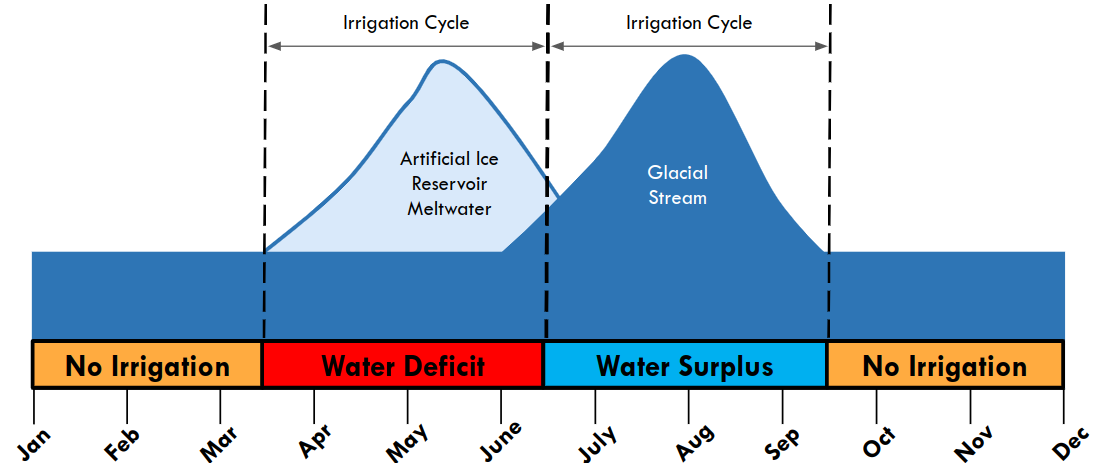
\includegraphics[width=12cm]{Figures/irrigation_cycles.png}

\caption{Seasonal variation in the availability of irrigation water. The graph highlights the crucial role of
AIRs in bridging the critical gap in water availability. Adapted from: \cite{nusserLocalKnowledgeGlobal2016}}

\label{fig:irrigation_cycles}
\end{figure}

Cryosphere-fed irrigation networks in arid mountain regions are completely dependent on timely availability of
meltwater from glaciers, snow and permafrost \citep{immerzeelImportanceVulnerabilityWorld2020,
farhanHydrologicalRegimesConjunction2015, tveitenGlacierGrowingLocal2007}. With the accelerated decline of
glaciers due to climate change \citep{nusserLocalKnowledgeGlobal2016}, these regions are experiencing water
scarcity particularly during the spring season \citep{norphelSnowWaterHarvesting2015,
mukhopadhyayReevaluationSnowmeltGlacial2015} (see Fig. \ref{fig:irrigation_cycles}). This seasonal water
scarcity makes it essential to provide supplementary irrigation in order to sustain agricultural output and take
advantage of the complete growing season \citep{nusserLocalKnowledgeGlobal2016, vincentEnergyClimateChange2009}.

To cope with this recurrent water scarcity, villagers in the region of Ladakh have developed two types of
artificial ice reservoirs (AIRs): ice stupas and ice terraces.  All these types of ice reservoirs capture water
in the autumn and winter, allowing it to freeze, and hold it until spring, when it melts and flows down to
fields \citep{ipccChapterHighMountain2019, vinceGlacierMan2009, clouseLadakhArtificialGlaciers2017,
nusserSociohydrologyArtificialGlaciers2019}. In this way, they retain a previously unused portion of the annual
flow and facilitate its use to supplement the decreased flow in the following spring (see Fig.
\ref{fig:irrigation_cycles}). This study focuses on the form of AIRs locally called as ice stupas.

Over the past decade, several ice stupas have been built to supplement irrigation water supply of mountain
villages in India \citep{wangchukIceStupaCompetition2020, palmerStoringFrozenWater2022,
aggarwalAdaptationClimateChange2021}, Kyrgyzstan \citep{bbcnewsBrightArtificialGlacier2020} and Chile
\citep{reutersConservationistsChileAim2021}. Despite this widespread adoption, only a few publications examine
the role of AIRs in the water resource management of these regions. None of these publications study AIRs
outside Ladakh. Moreover, the published quantifications of the water storage capacity of AIRs just in Ladakh
also vary widely between these studies \citep{norphelSnowWaterHarvesting2015, baglaArtificialGlaciersHelp1998}.

Quantifying the water storage capacity of AIRs is not straightforward since the formative processes of AIRs are
complex. These processes are controlled by local topography, meteorology and construction strategies used. Since
AIRs are ice structures with similar surface processes like glaciers, glacier models could be used to quantify
meteorological influences. However, due to their limited size, and comparatively more variable surface area,
this assessment requires a modelling approach which is optimally constrained with comprehensive data from
in-situ field measurements. Moreover, a spirit of improvisation guides the design and construction of AIRs
making it difficult to make quantitative comparison from site to site.  

This thesis fulfills these requirements as it provides a new set of AIR-specific volume and area measurements
from drone flights along with meteorological data during the construction period. All these datasets were
produced through construction strategies using fountain systems that are quantified via in-situ observations of
the fountain characteristics and discharge rate measurements. This thesis also provides a one-dimensional AIR
model which is calibrated and validated with several AIR datasets from locations with different meteorological
conditions and different fountain systems. While this thesis reviews published AIR research and presents a
comprehensive quantitative study of their water storage potential, we acknowledge that substantial additional
knowledge is held by farming communities building these structures since mid-1800s.

\begin{figure}[t]
\centering
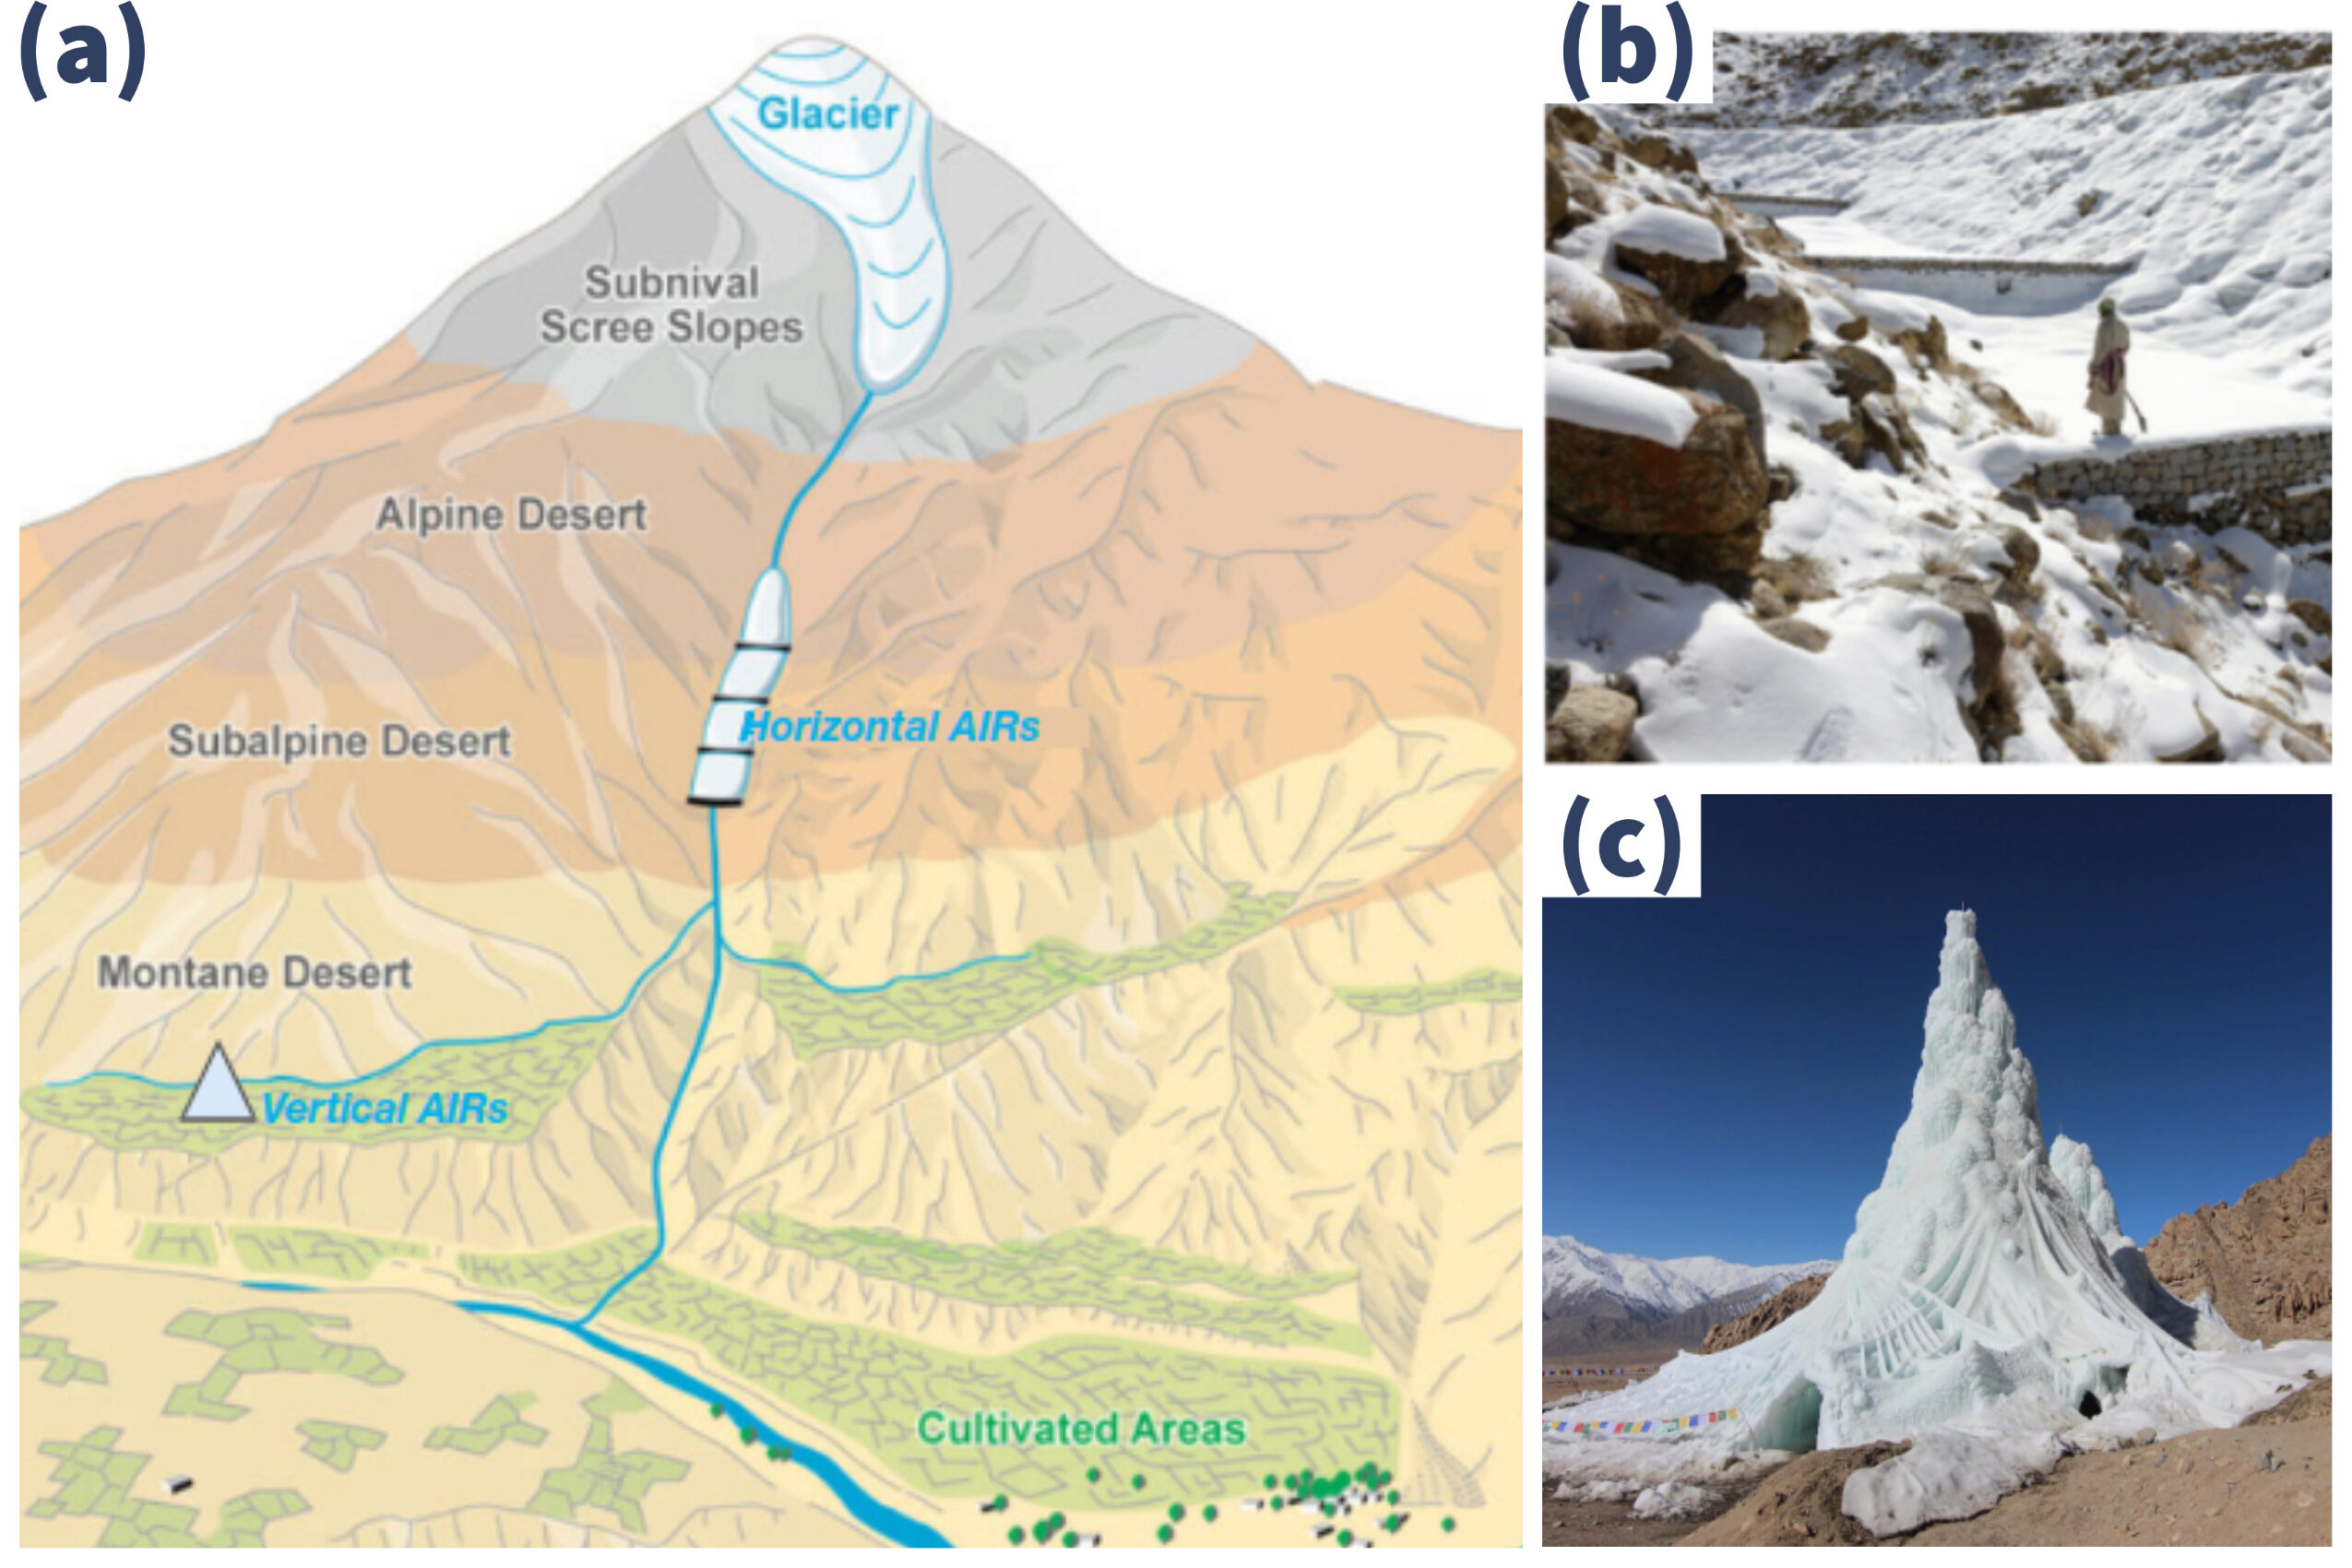
\includegraphics[width=12cm]{Figures/AIR_forms.jpg}

\caption{(a) Schematic overview of the position of artificial ice reservoirs. These constructions are located at
  altitudes between the glaciers and the irrigation networks in the cultivated areas. (b) Ice terraces at 3900
  m, located above the village of Nang, Ladakh. The cascade is composed of a series of loose masonry walls
  ranging in height from 2 to 3 $m$, which help freeze water for storage. (c) Ice stupas at 3600 m, located
above the village of Phyang, Ladakh. They are made using fountain systems. Adapted from:
\cite{nusserLocalKnowledgeGlobal2016}}

\label{fig:AIRforms}
\end{figure}

\section{Nomenclature and Classification}

In spite of the popularity of the term "artificial glacier", we deliberately use the term "ice reservoir" since
it conveys character and function of these structures more accurately
\citep{nusserSociohydrologyArtificialGlaciers2019}. Man-made ice structures typically have a lifetime in the
order of months and a size million times smaller than typical glaciers. Therefore, any comparison between these
ice structures can be misleading. Since glaciers are considered as natural ice reservoirs, we use the
terminology artificial ice reservoirs (AIRs) to distinguish man-made ice structures described in this thesis. 

A spirit of improvisation guides the construction strategy of AIRs making it difficult to classify them.
However, it has been found that construction strategies using fountain systems form AIRs which tend towards a
conical shape and those without form flat sheets of ice. Therefore, this thesis classifies all the AIRs produced
based on whether or not they use fountain systems. AIRs using fountain systems are called "ice stupas" and those
without are called "ice terraces" since this terminology denotes the resulting shape of the respective AIRs
appropriately.

\section{Objectives}

The main objective of this thesis is to quantify the water storage potential of AIRs based on the construction
site and fountain chosen. 

An integrated study approach including field measurements and modelling is applied to answer the following
research questions: 

\begin{enumerate}

\item What is the influence of construction location and fountain characteristics on AIR volume evolution? 

\item How can ice stupa fountain systems be engineered to reduce water loss and maintenance of AIRs?

\end{enumerate}

An energy and mass balance model for artificial ice reservoirs was set up to answer the first research question
(paper I and II). Since in-situ measurements were required to run this model, a measurement campaign was
executed in Switzerland and India during the past 4 winters. These datasets provided the necessary input,
calibration and validation data to model the evolution of AIRs and study their sensitivity to meteorological
conditions and fountain characterestics (paper II). 

Two weather-sensitive construction strategies were developed to answer the second research question. These
construction strategies employed fountains whose discharge rate was regulated by automation system using the AIR
model developed before. Their advantages and disadvantages over traditional construction strategy are quantified
in paper III.

\section{Structure}

Chapter 1 introduces the motivation of this work and provides a summary of the state of knowledge about AIRs
prior to this thesis. Chapter 2 describes the origins of this technology as a religious practice. Chapter 3
gives an overview about the study sites and introduces the different field techniques applied. The influence of
the construction location through its meteorological and topographical conditions are presented in Chapter 4.
The engineering design of AIR technologies are showcased in Chapter 5 along with suggestions for their
improvement. Chapter 6 concludes the thesis with a synthesis and future outlook. Papers I, II and III are
included in the Appendix.


 % Introduction

\chapter{Religion of ice reservoirs}

For centuries, in the Himalayan mountain ranges, local cultures have believed that glaciers are alive. And
what’s more, that certain glaciers can have different genders including male and female. These people ‘breed’
new glaciers by grafting together—or marrying—fragments of ice from male and female glaciers, then covering them
with charcoal, wheat husks, cloths, or willow branches so they can reproduce in privacy. These glacierets
transform into fully active glaciers that grow each year with additional snowfall. Those then serve as lasting
reserves of water that farmers can use to irrigate their crops. Over the years, these practices have inspired
other cultures, where people are creating their own artificial ice reservoirs (AIRs) and applying them to solve
serious modern challenges around water supplies.

\section{An old history}

According to legend, when the people of Baltistan learnt of the Mongol army advancing towards
them from the north in the early 13th century, they came up with an ingenious way to stop them. As the inhabited
valleys were only accessible through narrow passes, they decided to block the entry way by building a glacier.
This successfully prevented the Mongol invasion and, crucially, it also solved the locals’ other big problem:
water scarcity.

\section{The marriages of glaciers}

The people of Gilgit Baltistan believe that glaciers are living entities. That’s why a combination of female and
male ice was absolutely necessary. The male glacier – called ‘po gang’ locally – gives off little water and
moves slowly, while a ‘female glacier’ – or ‘mo gang’ – is a growing glacier that gives off a lot of water.

The glaciers that people help to grow are the fruit of the sacred union between a mother glacier and a father
glacier. They get married and have offspring. The selection of an appropriate site for this marriage is of
utmost importance, and a suitable spot must fulfil a list of conditions. It should be located at an altitude of
at least 4000 or 5000 metres above sea level; it should be on a gentle slope, where it should have minimal
exposure to sunlight, thus a north-facing mountain side is preferable. For most of the expert glacier grafters,
the presence of permafrost or ice on the site is another key requirement. 

Once a suitable spot is selected, the expedition can be planned. The bride and the groom – the female and the
male glacier, preferably from different villages – are chosen and the marriage can be planned. The glacier
grafting usually takes place in November, when the local temperatures oscillate around zero. A 12-man party
carries the pieces of female ice in woven baskets, another 12 men carry the male ice, the water drawn from the
Indus river is carried traditionally in 12 gourd bottles, but sometimes clay pots or goatskins are also
required, as well as charcoal and wheat husks or sawdust, which act as insulators for the ice. The last
ingredient is salt, which, according to some glacier grafters, helps protect the new glacier from impurities.
The bride and groom party walk from different sites and meet in a certain spot to climb together to the glacier
growing site, but no greetings are exchanged, as the people involved in the ceremony must remain silent until
the ice is deposited in its new home. They walk continuously without having a break, but if the distance is too
much and rest is required, they do not put their loads on the ground, instead hanging the baskets on trees, or
on walking sticks if nothing else is available. Each man has to carry around 15 to 25 kilograms of ice, walking
in cold air, silently up the mountains, for a day or more. Once they reach the glacier growing site, they
deposit their valuable loads. The ice lumps and water bottles are placed in between the boulders, or in a small
cave, or sometimes in a specially dug pit, and covered with layers of salt, charcoal and sawdust. The silence is
broken as religious leaders recite verses of the Quran and say prayers for the success of the glacier marriage
and for protection from the djinns. Once the male and female glaciers are placed in their new home and covered,
a man from the party of glacier grafters stands up and offers his life for the success of the process. His
symbolic sacrifice is matched by the actual sacrifice of a goat – its meat is distributed to a charity, because
prayers are more likely to be answered if accompanied by an act of charity. They will not visit the place for at
least three years, so as not to disturb the glacier. It is said that a person who disturbs the glacier before
its maturation will die. The celebrations continue in the village with traditional songs and prayers, alongside
festive food and the joy of the accomplished mission.

\section{From folklore to science}

Myths, legends and superstitions are ways of knowing. But they need to be translated to the language of science.
However, when it comes to past projects, there is only anecdotal evidence available.

According to Ingvar Tveiten, a researcher from Norway, the account of the glacier development process presented
by a glacier grafter from Balghar bears a strong resemblance to the definition of the formation of rock
glaciers. According to a description by a Balghar local: “First the ice slips down into the rocks where it grows
roots. Then it starts to break the rocks bringing them up. Then the glacier comes forward. This has happened
where they did the glacier growing.” Tveiten, who conducted field research in Baltistan, concludes that “glacier
growing is typically performed […] in a terrain that is conducive to the accumulation of snow by avalanching and
snow slips. The presence of permafrost at these locations is likely to contribute to ice accumulating […] Thus,
glacier growing is conducted at locations which are already very prone to ice accumulation, and may explain why
glacier growing is perceived to work.” Here it is, traditional knowledge translated into the language of
science.

Even the choice of the glacier grafting site suggests that the technique was developed as a result of the local
people’s deep understanding of local environmental processes. The view of glaciers as animate implies that
humans can influence on the lives of glaciers, just as glaciers can influence on the lives of people.

 % Background Theory

\chapter{Science of ice reservoirs}

This chapter provides the methodology used to estimate the ice volume evolution and water-use efficiency of
AIRs. The equations governing the mass and energy balance of vertical AIRs (or Icestupas) is explained along
with the associated datasets required for forcing, calibration and validation of this AIR model.

In a first step, the influence of the chosen location and fountain used was quantified by feeding weather and
fountain data to an energy balance model and validating the ice volume estimates produced with volume
observations from drone flights. In a second step, the model was extended to serve as a tool for recommending
discharge rates and identifying favourable construction locations worldwide.

\section{Study sites and data}

\subsection{Study sites}

We chose two villages in the Swiss Alps and the Indian Himalayas called Guttannen and Gangles to collect the
required datasets described above. These two locations exhibit drastically different ice volume evolution (see
Fig. \ref{fig:2AIRs}) owing to their latitude, longitude and altitude differences. The corresponding datasets
were categorised based on the construction strategy used, prefix of the country and the suffix of the winter
season. The construction strategies are distinguished based on whether they used weather-sensitive approaches to
regulate water supply. Those that did were codenamed automated construction strategy whereas the rest were
codenamed traditional construction strategy. In total, five AIRs were studied in these two locations across
three winters (see Table). Only one was built in Gangles. The rest were built in Guttannen. All except one
construction campaign used traditional construction strategies. Therefore, traditional AIRs are referred to
without explicitly specifying their construction strategy henceforth.

\begin{figure}
  \centering
	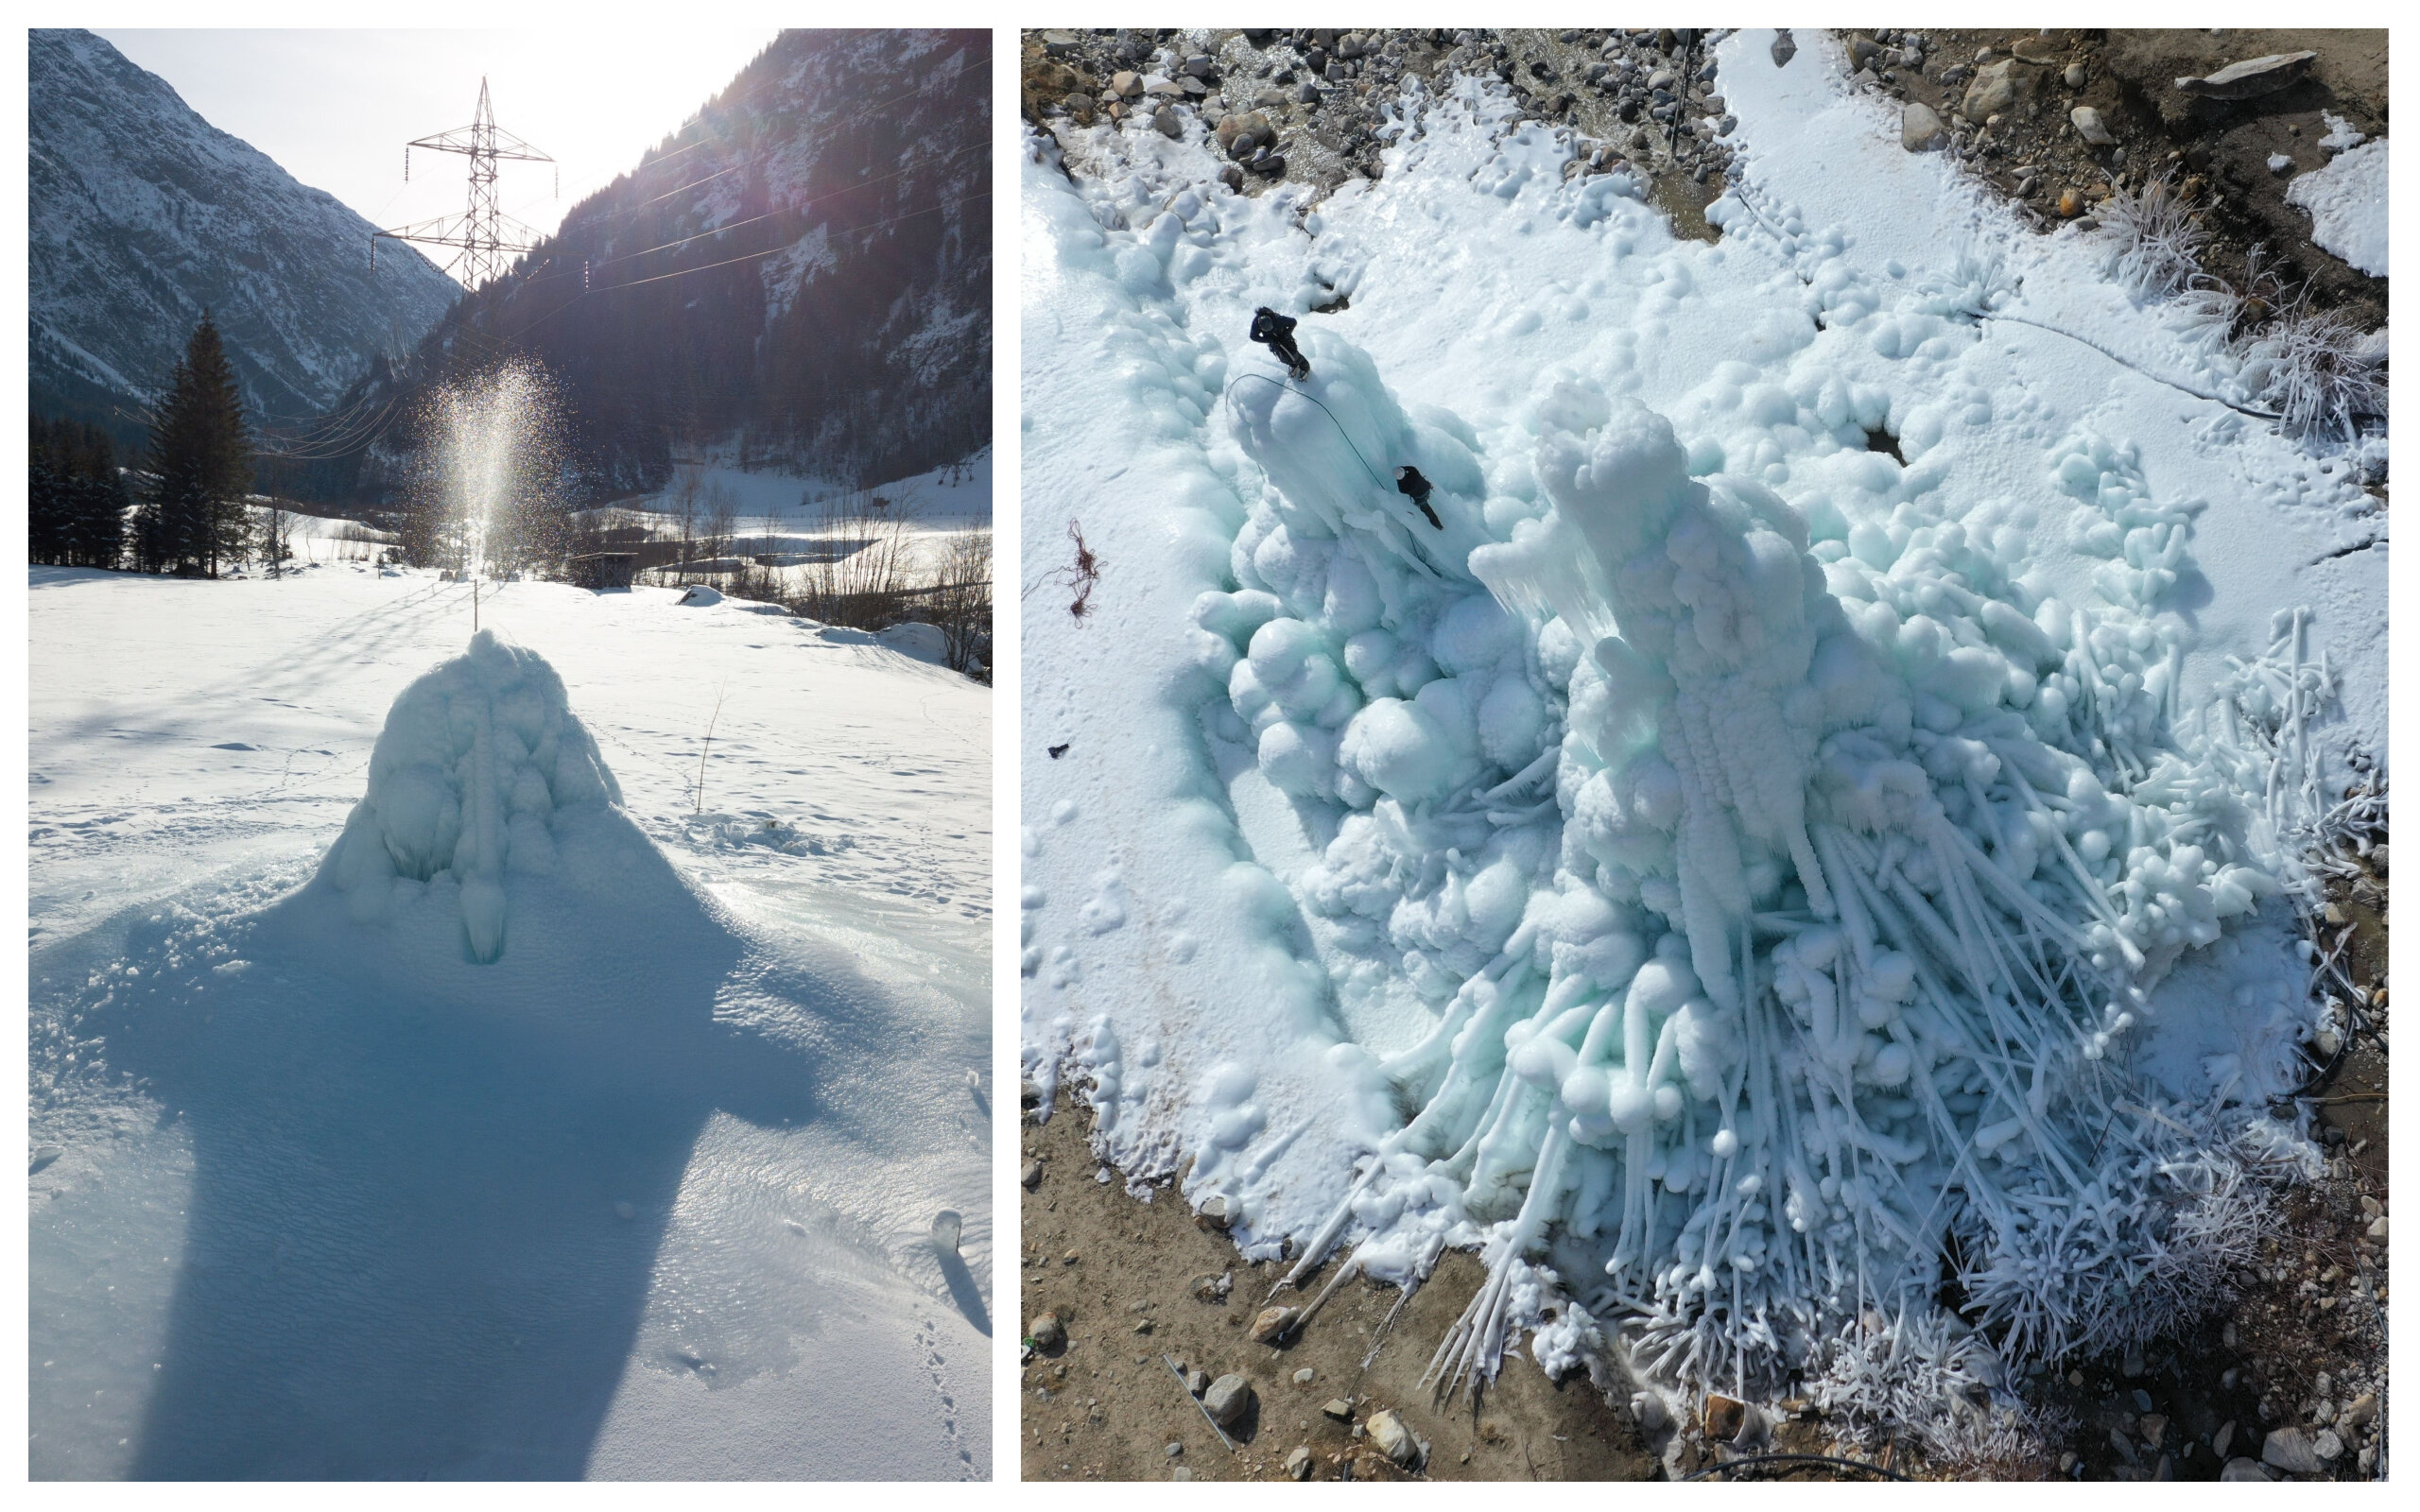
\includegraphics[width=12 cm]{Figures/2AIRs.jpg}
  \caption{The Swiss and Indian AIRs were 5 $m$ and 13 $m$ tall on January 9 and March 3, 2021 respectively. Picture
credits: Daniel Bürki (left) and Thinles Norboo (right)} 
\label{fig:2AIRs} 

\end{figure}

The Guttannen site (46.66 $\degree$N, 8.29 $\degree$E) is situated in the Berne region, Switzerland and has an
altitude of 1047 $m$ a.s.l. In the winter (Oct-Apr), mean daily minimum and maximum air temperatures vary
between -13 and 15 $\degree C$. Clear skies are rare, averaging around 7 days during winter. Daily winter
precipitation can sometimes be as high as 100 $mm$. These values are based on 30 years of hourly historical
weather data measurements \citep{meteoblueClimateGuttannen2021}. Several AIRs were constructed by the Guttannen
Bewegt Association, the University of Fribourg and the Lucerne University of Applied Sciences and Arts during
the winters of 2020-22.

The Gangles site (34.22 $\degree$N, 77.61 $\degree$E) is located around 20 km north of Leh city in the Ladakh
region, lying at 4025 $m$ a.s.l.. The mean annual temperature is $5.6 \, \degree C$, and the thermal range is
characterized by high seasonal variation. During January, the coldest month, the mean temperature drops to $-7.2
\, \degree C$. During August, the warmest month, the mean temperature rises to $17.5 \, \degree C$
\citep{nusserIrrigationDevelopmentUpper2012}. Because of the rain shadow effect of the Himalayan Range, the mean annual precipitation in
Leh totals less than 100 $mm$, and there is high interannual variability. Whereas the average summer rainfall
between July and September reaches 37.5 $mm$, the average winter precipitation between January and March amounts
to 27.3 $ mm$ and falls almost entirely as snow. AIRs were constructed here as part of the Ice Stupa Competition
by the Himalayan Institute of Alternatives, Ladakh (HIAL). 


\subsection{Meteorological data}

Air temperature, relative humidity, wind speed, pressure, longwave and global shortwave radiation are required
to calculate the surface energy balance of an AIR. The study period starts when the fountain was first switched
on and ends when the respective AIR melted completely. These two dates are denoted as start and expiry dates
henceforth. Each AIR is abbreviated based on the country code of the study site with the year of its expiry
date. The resulting dataset highlights the difference in meteorological influences driving ice volume evolution
in the two study sites (see Table \ref{tab:Observations}).


\begin{table}
  \centering
  \caption{Summary of the weather observations for AIRs built during the 2020-21 winter season. 
The weather measurements are shown using their mean ($\mu$) and standard deviation ($\sigma$) during the study
period as $\mu \pm \sigma$. }

	\label{tab:Observations}
	\begin{tabular}{|lllll|}
		\toprule
		\textbf{Name}               & \textbf{Symbol} & \textbf{IN21} & \textbf{CH21} & \textbf{Units}   \\ \midrule
		Air temperature             & $T_a    $       & $0 \pm 7$     & $2 \pm 6$     & $\degree C$      \\
		Relative humidity           & $RH     $       & $35 \pm 20$   & $79 \pm 18$   & \%               \\
    Wind speed                  & $v_a        $   & $3 \pm 1$     & $2 \pm 2$     & $m/s$            \\
		Direct Shortwave            & $SW_{direct} $  & $246 \pm 333$ & $80 \pm 156$  & $W\,m^{-2}$      \\
		Diffuse Shortwave           & $SW_{diffuse}$  & $0 \pm 0$     & $58 \pm 87$   & $W\,m^{-2}$      \\
		Hourly Precipitation        & $ppt        $   & $0 \pm 0$     & $139 \pm 457$ & $mm$             \\
		Pressure                    & $p_a         $  & $623 \pm 3$   & $794 \pm 9$   & $hPa$            \\\bottomrule
	\end{tabular}
\end{table}

\subsection{Fountain observations}

The fountain consists of a pipeline and a nozzle. The pipeline has three attributes, namely : discharge rate
($Q$), height ($h$) and water temperature ($T_F$). Discharge rate represents the discharge rate of the water in
the fountain pipeline. Height denotes the height of the fountain pipeline installed. Fountain water temperature
is the temperature of water droplets produced by the fountain.

The fountain nozzle has three characteristics, namely : the aperture diameter ($dia$), the spray radius ($r$)
and pressure loss ($P$) . Spray radius denotes the observed ice radius formed from the fountain water droplets.
Pressure loss denotes the loss of water head caused due to the fountain nozzle.

\subsection{Drone flights}

\begin{table}
  \centering
  \caption{List of all the studied AIRs. The study period starts when the fountain was first switched on
  (denoted as Start Date) and ends when the respective AIR either melted or broke into several ice blocks
(denoted as Expiry Date). }

	\label{tab:AIRs}
	\begin{tabular}{|lllll|}
		\toprule
		\textbf{Name}     & \textbf{Start Date} & \textbf{Expiry Date} & \textbf{No. of flights} & \textbf{Spray radius} \\ \midrule
    Traditional CH20  &  & & 2 & \\
    Traditional CH21  & Nov 22 2020   & May 10 2021 & 8 & 6.9 $m$ \\
    Traditional IN21  & Jan 18 2021   & June 20 2021 & 6 & 10.2 $m$ \\
    Traditional CH22  & Dec 8 2021 & April 12 2022 & 8 & \\
		Automated CH22  &  Dec 8 2021 & April 12 2022 & 6 & \\ \bottomrule
	\end{tabular}
\end{table}

Several photogrammetric surveys were conducted for each of the AIRs. The details of these surveys and the
methodology used to produce the corresponding outputs are explained in paper I. The digital elevation models
(DEMs) generated from the obtained imagery were analysed to document the ice radius, the surface area and the
volume of the ice structures. Ice radius measurements of drone flights which observed either an increase in AIR
circumference or volume were averaged to determine the fountain's spray radius. The number of drone surveys
conducted for each of the AIRs and the corresponding spray radius observed is shown in Table \ref{tab:AIRs}. 

\section{AIR Model}

A bulk energy and mass balance model is used to calculate the amounts of ice, meltwater, water vapour and
wastewater of the AIR. In each hourly time step, the model uses the AIR surface area, energy balance and mass
balance calculations to estimate its ice volume, surface temperature and wastewater as shown in Fig.
\ref{fig:schema} .

\begin{figure}
	\begin{center}
		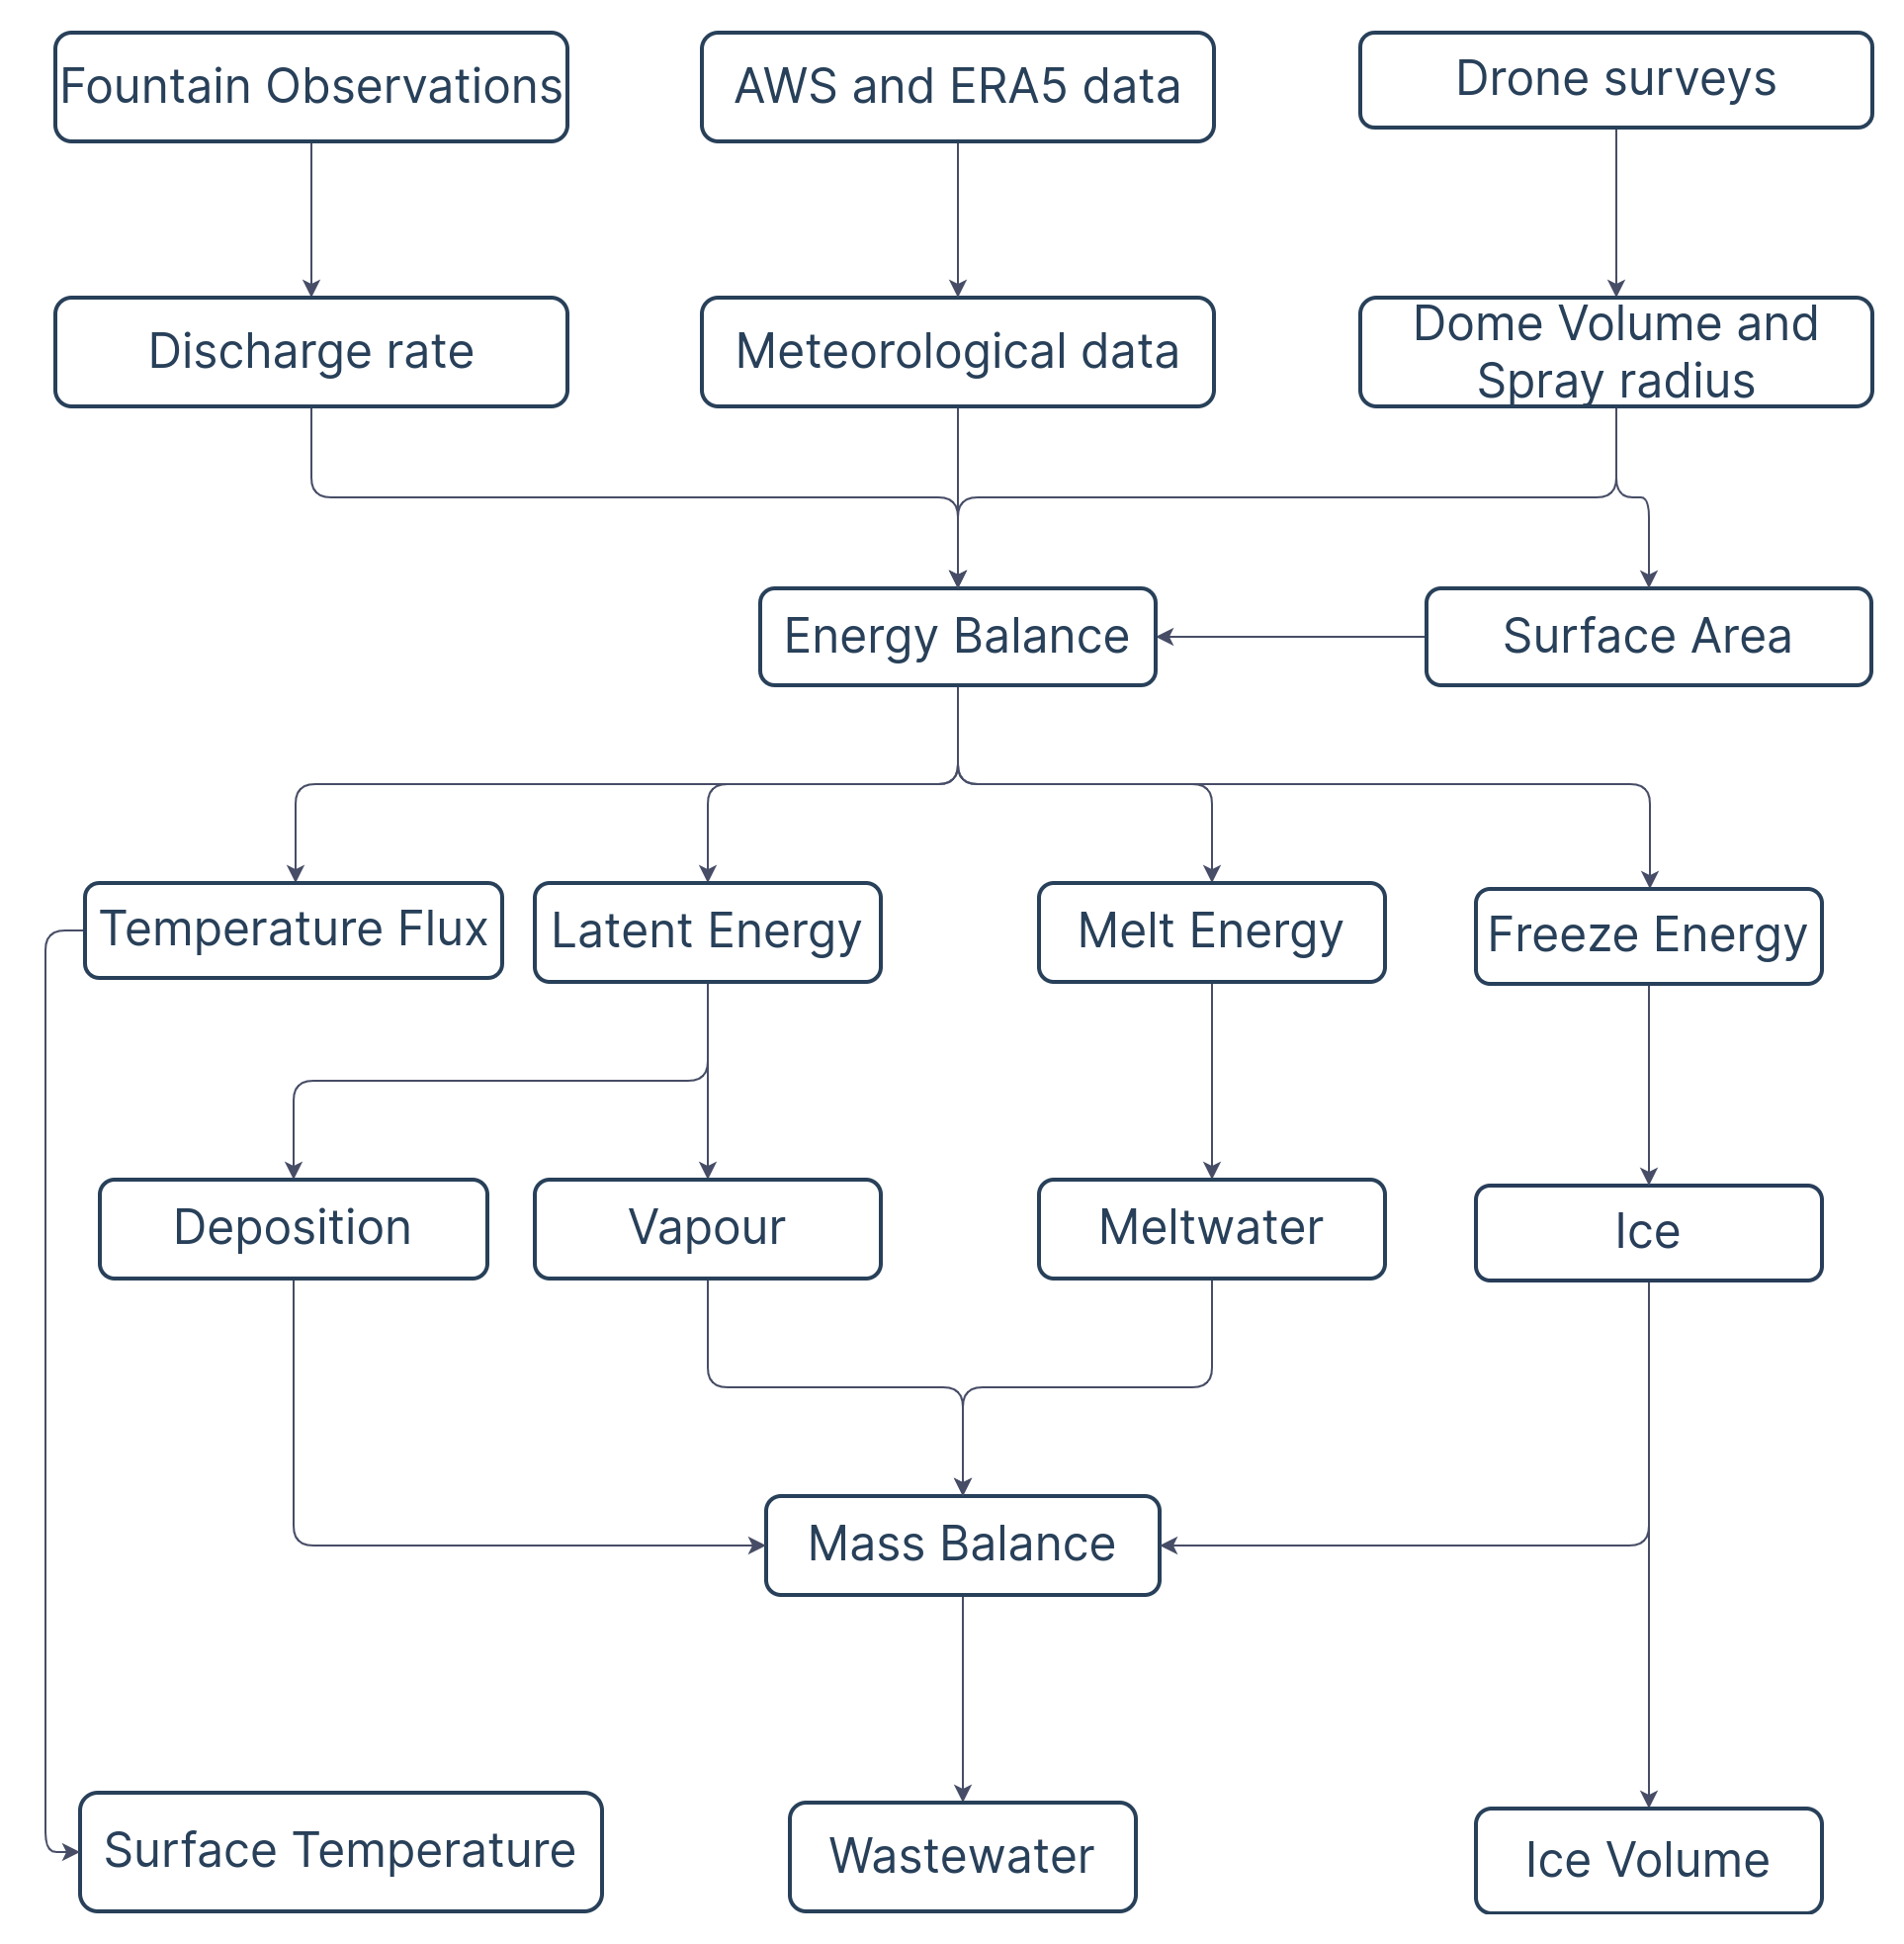
\includegraphics[width=10 cm]{Figures/Figure_3.jpg}
	\end{center}
	\caption{Model schematic showing the workflow used in the model at every time step. }
	\label{fig:schema}
\end{figure}

\subsection{Surface area calculation} \label{sec:shape}

The model assumes the AIR shape to be a cone and assigns the following shape attributes:

\begin{subequations}

	\begin{align}
		\label{eq:A}
		A_{cone}^i & = \pi \cdot r_{cone}^i \cdot \sqrt{{(r_{cone}^i)}^2 + {(h_{cone}^i})^ 2} \\
		\label{eq:V}
		V_{cone}^i & = \pi/3 \cdot {(r_{cone}^i)}^2 \cdot h_{cone}^i                                         \\
		\label{eq:thickness}
		j_{cone}^i & =\frac{\Delta M_{ice}^i}{\rho_{water}* A_{cone}^i}
	\end{align}
\end{subequations}

where $i$ denotes the model time step, $r_{cone}^i$ is the radius; $h_{cone}^i$ is the height; $A_{cone}^i$ is
the surface area; $V_{cone}^i$ is the volume and $j_{cone}^i$ is the AIR surface normal thickness change as shown
in Fig. \ref{fig:shape}. $M_{ice}^i$ is the mass of the AIR and $\Delta M_{ice}^i = M_{ice}^{i-1} -
M_{ice}^{i-2}$. Henceforth, the equations used display the model time step superscript $i$ only if it is different
from the current time step.

AIR density can be defined as:

\begin{equation}
  \rho_{cone} = \frac{M_{F} + M_{dep} + M_{ppt}}{(M_{F} + M_{dep})/\rho_{ice} + M_{ppt}/\rho_{snow}}
\end{equation}

where $M_F$ is the cumulative mass of the fountain discharge; $M_{ppt}$ is the cumulative precipitation;
$M_{dep}$ is the cumulative accumulation through water vapour deposition; $\rho_{ice}$ is the ice density (917
$kg\,m^{-3}$) and $\rho_{snow}$ is the density of wet snow (300 $kg\,m^{-3}$) taken from
\cite{cuffeyPhysicsGlaciers2010} .

AIR volume can also be expressed as:

\begin{equation} V_{cone} =\frac{M_{ice}} {\rho_{cone}} \label{eq:V1} \end{equation}

The initial radius of the AIR is assumed to be $r_F$. The initial height $h_0$ depends on the dome volume
$V_{dome}$ used to construct the AIR as follows:

\begin{equation}
	h_{0} =  \Delta x + \frac{3 \cdot V_{dome}}{\pi \cdot (r_F)^2 }
	\label{eq:h0}
\end{equation}

where $\Delta x$ is the surface layer thickness (defined in Section \ref{sec:energy})

During the subsequent time steps, the dimensions of the AIR evolve assuming a uniform thickness change ($j_{cone}$)
across its surface area with an invariant slope $s_{cone} = \frac{h_{cone}}{r_{cone}}$ .  During these time
steps, the volume is parameterised using Eqn. \ref{eq:V} as:

\begin{equation} V_{cone} = \frac{\pi \cdot {(r_{cone})}^3
		\cdot s_{cone}}{3} \label{eq:V2} \end{equation}

We define the Icestupa boundary through its spray radius, i.e. we assume ice formation is negligible when $r_{cone} >
	r_{F}$. Combining Eqns. \ref{eq:V},  \ref{eq:V1}, \ref{eq:h0} and \ref{eq:V2}, the geometric evolution of the
Icestupa at each time step $i$ can be determined by considering the following rules:

\begin{equation} (r_{cone},\, h_{cone}) = \left\{ \begin{array}{ll} (r_F ,\, h_0)                                                                          & \textit{ if } i=0 \\
		(r_{cone}^{i-1},\, \frac{3 \cdot M_{ice}}{\pi \cdot \rho_{ice} \cdot {(r_{cone}^{i-1})}^2}) & \textit{ if }
		r_{cone}^{i-1} \geq r_{F} \textit{ and } \Delta M_{ice} > 0                                                     \\ (\frac{3 \cdot M_{ice}}{\pi \cdot \rho_{ice} \cdot s_{cone}})^{1/3} \cdot (1,\,  s_{cone}) &
		otherwise\end{array} \right.  \label{eq:A2} \end{equation}


\subsection{Energy balance calculation} \label{sec:energy}

\begin{figure}
	\begin{center}
		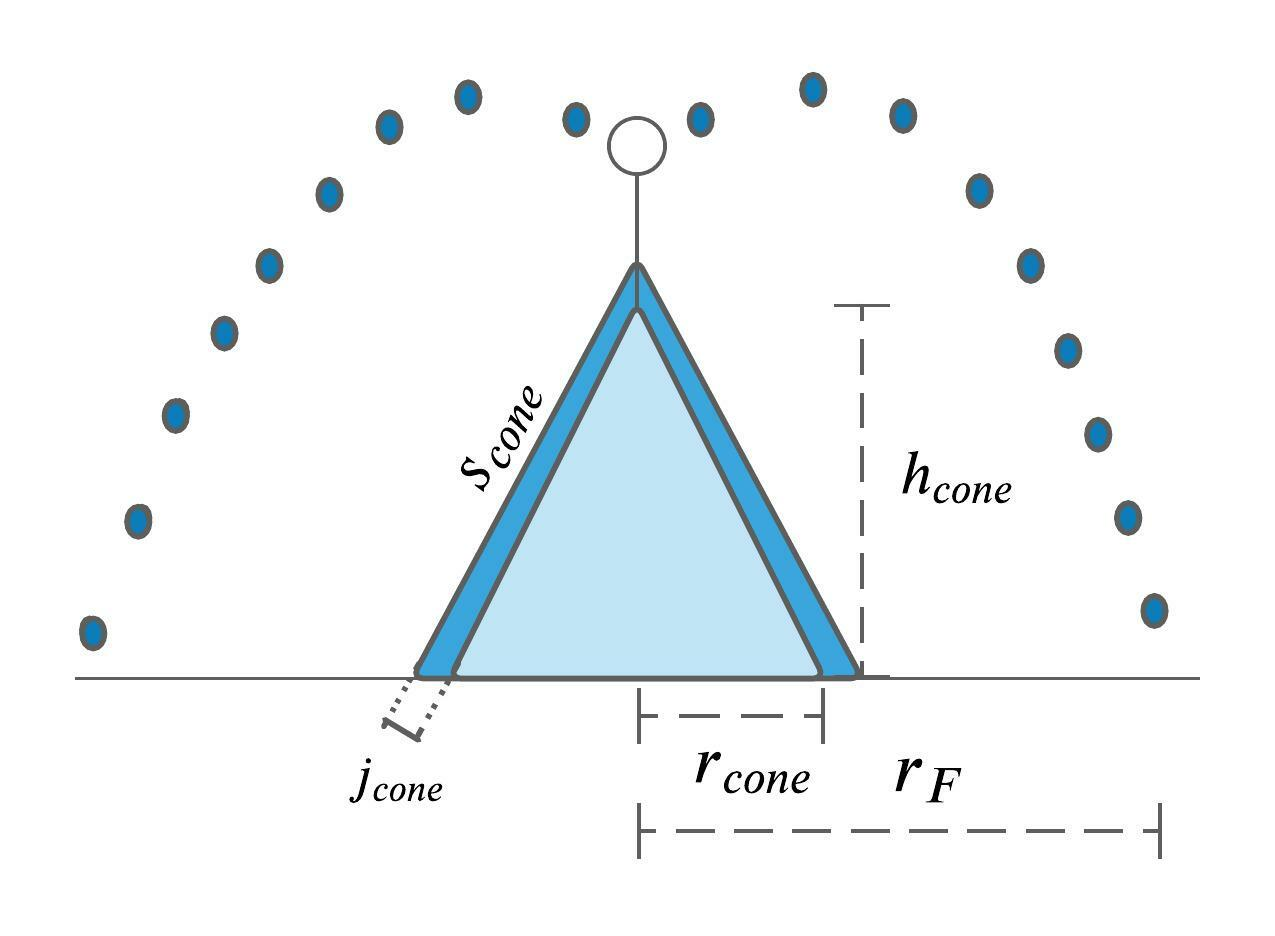
\includegraphics[width=10 cm]{Figures/Figure_4.jpeg}
	\end{center}
	\caption{Shape variables of the AIR. $r_{cone}$ is the radius, $h_{cone}$ is the height, $j_{cone}$ is the
		thickness change and $s_{cone}$ is the slope of the ice cone. $r_F$ is the spray radius of the fountain.}
	\label{fig:shape}
\end{figure}

We approximate the energy balance at the surface of an AIR by a one-dimensional description of energy fluxes
into and out of a (thin) layer with thickness $\Delta x$:

\begin{equation}
  \rho_{cone} \cdot c_{ice} \cdot \frac{\Delta T}{\Delta t} \cdot \Delta x = q_{SW} + q_{LW} + q_{L} + q_{S} + q_{F}+ q_{R} + q_{G}
	\label{eqn:EB}
\end{equation}

Upward and downward fluxes relative to the ice surface are positive and negative, respectively. The first term
is the energy change of the surface layer, which can be translated into a phase change energy should phase
changes occur. $q_{SW}$ is the net shortwave radiation; $q_{LW}$ is the net longwave radiation; $q_{L}$ and
$q_{S}$ are the turbulent latent and sensible heat fluxes. $q_{F}$ and $q_{R}$ represent the heat exchange of
the fountain water droplets and rain droplets with the AIR ice surface respectively. $q_{G}$ represents ground
heat flux between the AIR surface and its interior.

The density of the AIR $\rho_{cone}$ was parameterised as follows:

\begin{equation}
  \rho_{cone} = \frac{M_{F} + M_{dep} + M_{ppt}}{(M_{F} + M_{dep})/\rho_{ice} + M_{ppt}/\rho_{snow}}
\end{equation}

where $M_F$ is the cumulative mass of the fountain discharge; $M_{ppt}$ is the cumulative precipitation;
$M_{dep}$ is the cumulative accumulation through water vapour deposition; $\rho_{ice}$ is the ice density (917
$kg\,m^{-3}$) and $\rho_{snow}$ is the density of wet snow (300 $kg\,m^{-3}$) taken from
\cite{cuffeyPhysicsGlaciers2010} .

The energy flux acts upon the AIR surface layer, which has an upper and lower boundary defined by the atmosphere
and the ice body of the AIR, respectively. Here, we define the surface temperature $T_{ice}$ to be the modelled
average temperature of the icestupa surface layer.

\subsubsection{Net Shortwave Radiation \texorpdfstring{$q_{SW}$}{Lg}} \label{sec:SW}

The net shortwave radiation $q_{SW}$ is computed as follows:

\begin{equation} q_{SW} = (1- \alpha)\cdot (SW_{direct} \cdot f_{cone} + SW_{diffuse}) \label{eqn:SW} \end{equation}

where $SW_{direct}$ and $SW_{diffuse}$ are the direct and diffuse shortwave radiation, $\alpha$ is the
modelled albedo and $f_{cone}$ is the area fraction of the ice structure exposed to the direct shortwave
radiation.

The albedo varies depending on the water source that formed the current AIR surface layer. During the fountain
runtime, the albedo assumes a constant value corresponding to ice albedo. However, after the fountain is
switched off, the albedo can reset to snow albedo during snowfall events and then decay back to ice albedo. We
use the scheme described in \cite{oerlemansYearRecordGlobal1998} to model this process. The scheme records the
decay of albedo with time after fresh snow is deposited on the surface. $\delta t$ records the number of time
steps after the last snowfall event. After snowfall, albedo changes over a time step, $\delta t$ , as

\begin{equation} \alpha=\alpha_{ice}+(\alpha_{snow}-\alpha_{ice}) \cdot e^{(-\delta t)/\tau} \label{eqn:a}
\end{equation}

where $\alpha_{ice}$ is the bare ice albedo value (0.25), $\alpha_{snow}$ is the fresh snow albedo value (0.85)
and $\tau$ is a decay rate (16 $days$), which determines how fast the albedo of the ageing snow recedes back to
ice albedo. Discharge events decrease the decay rate by a factor of $\alpha_{ice}/\alpha_{snow}$. 

The solar area fraction $f_{cone}$ of the ice structure exposed to the direct shortwave radiation depends on the shape
considered. Using the solar elevation angle $\theta_{sun}$, the solar beam can be considered to have a vertical
component, impinging on the horizontal surface (semicircular base of the AIR), and a horizontal component
impinging on the vertical cross section (a triangle). The solar elevation angle $\theta_{sun}$ used is modelled
using the parametrisation proposed by \cite{woolfComputationSolarElevation1968}. Accordingly, $f_{cone}$ is determined as follows:

\begin{equation}
	\begin{split}
		f_{cone}& =\frac{(0.5 \cdot r_{cone} \cdot h_{cone}) \cdot cos \theta_{sun} +(\pi \cdot
			{(r_{cone})}^2/2) \cdot sin \theta_{sun} }{\pi \cdot r_{cone} \cdot ({(r_{cone})}^2+{(h_{cone})}^2)^{1/2}}\\
	\end{split}
	\label{eqn:f_{cone} }
\end{equation}

The diffuse shortwave radiation is assumed to impact the conical AIR surface uniformly.

\subsubsection{Net Longwave Radiation \texorpdfstring{$q_{LW}$}{Lg}} \label{sec:LW}

The net longwave radiation $q_{LW}$ is determined as follows:

\begin{equation}
	q_{LW}= LW_{in}-\sigma \cdot \epsilon_{ice} \cdot {(T_{ice}+ 273.15)}^4
	\label{eqn:LW}
\end{equation}

where $T_{ice}$ is the modelled surface temperature given in [$\degree C$],
$\sigma=5.67\cdot10^{-8}\,Jm^{-2}s^{-1}K^{-4}$ is the Stefan-Boltzmann constant, $LW_{in}$ denotes the incoming
longwave radiation and $\epsilon_{ice}$ is the corresponding emissivity value for the Icestupa surface (0.97).

The incoming longwave radiation $LW_{in}$ for the Indian site, where no direct measurements were available, is
determined as follows:

\begin{equation}
	LW_{in}=\sigma \cdot \epsilon_a \cdot {(T_a+ 273.15)}^4
	\label{eqn:LWin}
\end{equation}

here $T_a$ represents the measured air temperature and $\epsilon_a$ denotes the atmospheric emissivity. We
approximate the atmospheric emissivity $\epsilon_a$ using the equation suggested by \cite{brutsaertEvaporationAtmosphereTheory1982},
considering air temperature and vapor pressure (Eqn.  \ref{eqn:atm_e}). The vapor pressure of air over water and
ice was obtained using Eqn. \ref{eqn:vp}.  The expression defined in \cite{brutsaertDerivableFormulaLongwave1975} for clear skies
(first term in equation \ref{eqn:atm_e}) is extended with the correction for cloudy skies after
\cite{brutsaertEvaporationAtmosphereTheory1982} as follows:

\begin{equation}
	\epsilon_a=1.24 \cdot (\frac{p_{v,w}}{(T_a+273.15)})^{1/7}\cdot(1+0.22\cdot{cld}^2) \label{eqn:atm_e}
\end{equation}

with a cloudiness index $cld$, ranging from 0 for clear skies to 1 for complete overcast skies. For the Indian
site, we assume cloudiness to be negligible.

\subsubsection{Turbulent fluxes} \label{sec:Qs}

The turbulent sensible $q_{S}$ and latent heat $q_{L}$ fluxes are computed with the following expressions
proposed by \cite{garrattAtmosphericBoundaryLayer1992}:

\begin{equation}
	q_{S}=\mu_{cone}\cdot c_{a} \cdot \rho_{a} \cdot p_{a}/p_{0,a} \cdot \frac{\kappa^2 \cdot v_a \cdot
		(T_a-T_{ice})}{{(\ln{\frac{h_{AWS}}{z_{0}}})}^2}
	\label{eqn:qs}
\end{equation}

\begin{equation}
	q_{L}=\mu_{cone}\cdot 0.623 \cdot L_s \cdot \rho_{a}/p_{0,a} \cdot \frac{\kappa^2 \cdot
	v_a(p_{v,w}-p_{v,ice})}{{(\ln{\frac{h_{AWS}}{z_{0}}})}^2}
\end{equation}

where $h_{AWS}$ is the measurement height above the ground surface of the AWS (around $2\,m$ for all sites),
$v_a$ is the wind speed in [$m\,s^{-1}$], $c_a$ is the specific heat of air at constant pressure (1010 J
$kg^{-1} K^{-1}$), $\rho_{a}$ is the air density at standard sea level (1.29 $kg m^{-3}$), $p_{0,a}$ is the air
pressure at standard sea level (1013 $hPa$), $p_{a}$ is the measured air pressure, $\kappa$ is the von Karman
constant (0.4), $z_{0}$ is the surface roughness (3 $mm$) and $L_s$ is the heat of sublimation (2848
$kJ\,kg^{-1}$).  The vapor pressure of air with respect to water ($p_{v,w}$) and with respect to ice
($p_{v,ice}$) was obtained using the formulation given in \cite{huangSimpleAccurateFormula2018} :

\begin{equation}
	\begin{split}
		p_{v,w}&=e^{\frac{(34.494 - \frac{4924.99}{T_{a} + 237.1})}{(T_a + 105)^{1.57} \cdot 100}} \cdot \frac{RH}{100} \\
		p_{v,ice}&=e^{\frac{(43.494 - \frac{6545.89}{T_{ice} + 278})}{(T_{ice} + 868)^{2} \cdot 100}} \\
	\end{split} \label{eqn:vp}
\end{equation}

The dimensionless parameter $\mu_{cone}$ is an exposure parameter that deals with the fact that AIR has a rough
appearance and forms an obstacle to the wind regime. This factor accounts for the larger turbulent fluxes due to
the roughness of the surface \citep{oerlemansBriefCommunicationGrowth2021}, and is a function of the AIR slope
as follows:

\begin{equation}
	\mu_{cone} = 1 + \frac{s_{cone}}{2}
\end{equation}

A possible source of error is the fact that wind measurements from the horizontal plane at the AWS are used,
which might be different from those on a slope. However, without detailed datasets from the AIR surface, we
retain this assumption.

\subsubsection{Fountain discharge heat flux \texorpdfstring{$q_{F}$}{Lg} } \label{sec:heatflux}

The fountain water temperature $T_F$ is assumed to cool to 0 $\degree C$ after contact with the ice surface.
$T_F$ is equal to the measured source water temperature. But during time periods when the ambient temperature is
subzero, $T_F$ is assumed to be 0 $\degree C$. Thus, the heat flux caused by this process is:

\begin{equation}
	q_{F} = \left\{ \begin{array}{ll}
		\frac{ \Delta M_F \cdot c_{water} \cdot T_F}{\Delta t \cdot A_{cone}} & \textit{ if } T_{temp} > 0 \\
		0   & \textit{ otherwise}
	\end{array} \right.
\end{equation}

with $c_{water}$ as the specific heat of water (4186 J $kg^{-1} K^{-1}$).

\subsubsection{Rain heat flux \texorpdfstring{$q_{R}$}{Lg} }

The influence of rain events on the albedo and the energy balance was assumed to be similar to that of discharge
events. However, the water temperature of a rain event was assumed to equal to the air temeperature. Accordingly,
the heat flux generated due to a rain event was equal to:

\begin{equation}
  q_{R} = \frac{ \Delta M_{ppt} \cdot c_{water} \cdot T_a}{\Delta t \cdot A_{cone}}
	\label{eqn:qR}
\end{equation}

\subsubsection{Bulk Icestupa heat flux \texorpdfstring{$q_{G}$}{Lg}} \label{sec:Bulkflux}

The bulk Icestupa heat flux $q_{G}$ corresponds to the ground heat flux in normal soils and is caused by the
temperature gradient between the surface layer ($T_{ice}$) and the ice body ($T_{bulk}$). It is expressed by
using the heat conduction equation as follows:

\begin{equation} q_{G} = k_{ice} \cdot (T_{bulk}-T_{ice}^{i-1})/l_{cone} \label{eqn:qG}    \end{equation}

where $k_{ice}$ is the thermal conductivity of ice (2.123 $W\, m^{-1}\,K^{-1}$) , $T_{bulk}$ is the mean
temperature of the ice body within the icestupa and $l_{cone}$ is the average distance of any point in the
surface to any other point in the ice body. $T_{bulk}$ is initialised as 0 $\degree C$ and later determined from
Eqn. \ref{eqn:qG} as follows:

\begin{equation} T_{bulk}^{i+1} = T_{bulk} - (q_{G} \cdot A \cdot \Delta t)/(M_{ice} \cdot c_{ice}) \end{equation}

Since AIRs typically have conical shapes with $r_{cone} > h_{cone}$, we assume that the center of mass of the cone
body is near the base of the fountain. Thus, the distance of every point in the AIR surface layer from the cone
body's center of mass is between $h_{cone}$ and $r_{cone}$. Therefore, we calculate $q_{G}$ assuming $l_{cone} = (r_{cone} +
	h_{cone})/2$.

\subsubsection{Phase changes}\label{sec:phase}

In this section, the numerical procedures to model phase changes at the surface layer are explained. Let
$T_{temp}$ be the calculated surface temperature. Therefore, Eqn. \ref{eqn:EB} can be rewritten as:

$$q_{total} =\rho_{ice} \cdot c_{ice} \cdot \frac{(T_{temp}-T_{ice})}{\Delta t} \cdot \Delta x$$

where $q_{total}$ represents the total energy available to be redistributed. Even if the numerical heat transfer
solution produces temperatures which are $T_{temp}>0\, \degree C$, say from intense shortwave radiation, the ice
temperature must remain at $T_{temp} = 0\, \degree C$. The ‘‘excess’’ energy is used to drive the melting
process. Moreover, the energy input is used to melt the surface ice layer, and not to raise the surface
temperature to some unphysical value. Similarly, for freezing to occur, three conditions are required. Firstly,
fountain water is present ($\Delta M_{F} > 0 $) and secondly the calculated temperature of the ice, $T_{temp}$,
is below $0\, \degree C$. However, these two conditions are not sufficient as the latent heat turbulent fluxes
can only contribute to temperature fluctuations. Therefore, an additional condition, namely, $(q_{total}-q_{L})
< 0$, is required. Depending on the above conditions, the total energy $q_{total}$ can be redistributed
for the melting ($q_{melt}$), freezing ($q_{freeze}$) and surface temperature change ($q_{T}$) processes as
follows:

\begin{equation}
	q_{total} = \left\{ \begin{array}{ll}
		q_{freeze} + q_{T} & \textit{ if } \Delta M_{F} > 0 \textit{ and } T_{temp} < 0 \textit{ and }(q_{total}-q_{L}) < 0 \\
		q_{melt} + q_{T}   & \textit{ otherwise}
	\end{array} \right.
\end{equation}

Henceforth, time steps when the the total energy is redistributed to the freezing energy are called freezing
events and the rest of the time steps are called melting events.


During a freezing event, the AIR surface is assumed to warm to $0 \degree C$. The available energy
$(q_{total}-q_{L})$ is further increased due to this change in surface temperature represented by the energy
flux:

$$q_{0} = \frac{\rho_{ice} \cdot \Delta x \cdot c_{ice} \cdot T_{ice}^{i-1}}{\Delta t}$$

The available fountain discharge ($\Delta M_{F}$) may not be sufficient to utilize all the freezing energy. At such times, 
the additional freezing energy further cools down the surface temperature. Accordingly, the surface energy flux
distribution during a freezing event can be represented as:

\begin{equation}
	(q_{freeze}, q_{T}) = \left\{ \begin{array}{ll}
		(\frac{\Delta M_{F} \cdot L_f
		}{A_{cone} \cdot \Delta t}
		, q_{total}+\frac{\Delta M_{F} \cdot L_f
		}{A_{cone} \cdot \Delta t})          & \textit{ if  } \Delta M_{F} \textit{ insufficient }\\
		(q_{total}-q_{L}+q_{0}, q_{L}-q_{0}) & \textit{ otherwise }                                                                      \\
	\end{array} \right.
\end{equation}

If $T_{temp} > 0 \degree C$, then energy is reallocated from $q_{T}$ to $q_{melt}$ to maintain surface
temperature at melting point. The total energy flux distribution during a melting event can be represented as:

\begin{equation}
	(q_{melt}, q_{T}) = \left\{ \begin{array}{ll}
		(0, q_{total})
    & \textit{ if } T_{temp} \leq 0 \\
		(\frac{T_{temp} \cdot \rho_{ice} \cdot c_{ice} \cdot \Delta x}{\Delta t}, q_{total}-\frac{T_{temp} \cdot \rho_{ice} \cdot c_{ice} \cdot \Delta x}{\Delta t}  ) & \textit{ if } T_{temp} > 0
	\end{array} \right.
\end{equation}


\subsection{Mass balance calculation}

The mass balance equation for an AIR is represented as:

\begin{equation}
	\frac{\Delta M_{F} + \Delta M_{ppt} + \Delta M_{dep}}{\Delta t} = \frac{\Delta M_{ice} +\Delta M_{water} +
		\Delta M_{sub} + \Delta M_{waste}}{\Delta t}  \\
	\label{eq:MB}
\end{equation}

where $M_{F}$ is the cumulative mass of the fountain discharge; $M_{ppt}$ is the cumulative precipitation;  $M_{dep}$ is the cumulative
accumulation through water vapour deposition; $M_{ice}$ is the cumulative mass of ice; $M_{water}$ is the cumulative
mass of melt water; $M_{sub}$ represents the cumulative water vapor loss by sublimation and $M_{waste}$ represents the
fountain wastewater that did not interact with the AIR. The left hand side of equation \ref{eq:MB} represents the rate of
mass input and the right hand side represents the rate of mass output for an AIR.

Precipitation input is calculated as shown in equation \ref{eq:ppt} where $\rho_{w}$ is the density of water (1000
$kg\,m^{-3}$), $\Delta ppt/ \Delta t$ is the measured precipitation rate in [$m\,s^{-1}$] and $T_{ppt}$ is the temperature threshold
below which precipitation falls as snow. Here, snowfall events were identified using $T_{ppt}$ as $1 \degree C$. Snow
mass input is calculated by assuming a uniform deposition over the entire circular footprint of the AIR.

The latent heat flux is used to estimate either the evaporation and condensation processes or sublimation and deposition
processes as shown in equation \ref{eq:vap}. During the time steps at which the surface temperature is below 0 $\degree C$ only
sublimation and deposition can occur, but if the surface temperature reaches 0 $\degree C$, evaporation and condensation
can also occur. As the differentiation between evaporation and sublimation (and condensation and deposition) when the
air temperature reaches 0 $\degree C$ is challenging, we assume that negative (positive) latent heat fluxes correspond
only to sublimation (deposition), i.e. no evaporation (condensation) is calculated.

Since we have categorized every time step as a freezing or melting event, we can determine the melting/freezing
rates and the corresponding meltwater/ice quantities as shown in equations \ref{eq:m_freeze/melt}, \ref{eq:mwat}
and \ref{eq:mcone}. Having calculated all other mass components, the fountain wastewater generated every
time step can be calculated using Eqn. \ref{eq:MB}.

\begin{subequations}
	\begin{align}
		\frac{\Delta M_{F}}{\Delta t} & = \left\{ \begin{array}{ll} \frac{60}{\rho_w \cdot \Delta t} \cdot d_F
			 & \textit{ if fountain is on} \\ 0 & \textit{ otherwise } \\\end{array} \right.                                             \\
		\label{eq:ppt}
		\frac{\Delta M_{ppt}}{\Delta t}                                    & = \left\{ \begin{array}{ll} \pi \cdot
        {(r_{cone})}^2 \cdot
			\rho_{w}\cdot \frac {\Delta ppt}{\Delta t} & \textit{ if } T_{a} < T_{ppt} \\ 0 & \textit{ if } T_{a} \geq T_{ppt} \\\end{array} \right.                                             \\
		\label{eq:vap}
		(\frac{\Delta M_{dep}}{\Delta t}, \frac{\Delta M_{sub}}{\Delta t}) & = \left\{ \begin{array}{ll} \frac{q_{L}
			\cdot A_{cone}}{L_s}\cdot (1,0)  & \textit{ if } q_{L} \geq 0 \\ \frac{q_{L}
			\cdot A_{cone}}{L_s}\cdot (0,-1) & \textit{ if } q_{L} < 0    \\\end{array} \right.                                             \\
		\label{eq:mwat}
		\frac{\Delta M_{water}}{\Delta t}                                  & = \frac{q_{melt} \cdot A_{cone} }{L_f}                                                   \\
	  \label{eq:m_freeze/melt}
    \frac{\Delta M_{freeze/melt}}{\Delta t} & = \frac{q_{freeze/melt} \cdot A_{cone} }{L_f} \\
		\label{eq:mcone}
		\frac{\Delta M_{ice}}{\Delta t}                                    & = \frac{q_{freeze}\cdot A_{cone} }{L_f} + \frac{\Delta M_{ppt}}{\Delta t} + \frac{\Delta
			M_{dep}}{\Delta t}- \frac{\Delta M_{sub}}{\Delta t}- \frac{\Delta M_{water}}{\Delta t}
	\end{align}
\end{subequations}

Considering AIRs as water reservoirs, their net water loss can be defined as:

\begin{equation} \textit{Net water losses} = \frac{M_{waste}+M_{sub}}{(M_F+M_{ppt}+M_{dep})} \cdot 100 \end{equation}


\section{Model extensions}

The AIR model presented above was extended in order to (a) recommend fountain scheduling strategies and (b)
improve its transferability to new locations.

\subsection{Discharge rate scheduler}

In this section, we focus on the description of the integration of fountain scheduling processes in the model.

Two types of fountain scheduling strategies are possible depending on the contraints of water supply and
favourable weather window in the respective location. Locations constrained by their available water supply
require water-sensitive fountain scheduling strategies and those constrained by the duration of favourable
weather windows require weather-sensitive fountain scheduling strategies. These two kinds of scheduled fountains
will be referred to as water-sensitive fountain and weather-sensitive fountain henceforth.

Water-sensitive fountains are expected to produce higher water use effiency whereas weather-sensitive fountains
are expected to produce higher ice volumes. Accordingly, we produce the discharge rate recommendations for these
two kinds of fountains through two sets of model forcing assumptions for the following three model variables:
(a) slope , (b) albedo and (c) cloudiness.  These two kinds of models will be referred to as ice volume
optimised model (IVOM) and water-use efficiency optimised model (WEOM) respectively. The slope variable
increases the shortwave radiation and sensible heat impact. The albedo variable decreases the shortwave
radiation impact. The cloudiness variable increases both the shortwave and the longwave radiation impact. We
associate the upper and lower bounds of these variables with the IVOM and WEOM versions depending on whether
they overestimate and underestimate the freezing rate of the AIR as shown in Table \ref{tab:assumptions}.

\begin{table}[]
\centering
\caption{Assumptions for the parametrisation introduced to simplify the model.}
\label{tab:assumptions}
\begin{tabular}{@{}lllll@{}}
\toprule
\textbf{Estimation of} & \textbf{Symbol} & \textbf{IVOM} & \textbf{WEOM} & \\ \midrule
\multicolumn{1}{|l}{Slope}        & $s_{cone}$ & $ 1 $ & $0$ & \multicolumn{1}{l|}{} \\ \midrule
\multicolumn{1}{|l}{Albedo} & $\alpha$ & $\alpha_{snow}$ & $\alpha_{ice}$ & \multicolumn{1}{l|}{} \\\midrule 
\multicolumn{1}{|l}{Cloudiness}  & $cld$ & $0$ & $1$ & \multicolumn{1}{l|}{} \\ \bottomrule
\end{tabular}
\end{table}

We apply the assumptions described in Table \ref{tab:assumptions} on the one-dimensional description of energy
fluxes through Eqn. \ref{eqn:EB}. The derivation of the individual energy and mass balance terms for the IVOM
and WEOM model versions are discussed in Paper III.

% \subsection{COSISTUPA: COSIPY based model with lower calibration requirements }
\subsection{Location classifier}

The model, in its current form, is not expected to perform well for locations where it has not been calibrated
for before. This limits its ability to identify and classify other favourable locations worldwide.

In this section, we showcase a strategy to improve the AIR model's transferability to new locations.
Specifically, in paper I, we highlight the sensitivity of the model to the surface layer thickness parameter.
This parameter requires prior calibration for better model performance. However, the dependence of the model on
this parameter can be removed if spatial temperature fluctuations across the ice structure are resolved.

Here we combine the AIR model with the COupled Snowpack and Ice surface energy and mass balance model in PYthon
(COSIPY) in order to remove the calibration requirements for model performance. COSIPY is typically used for
modelling distributed snow and glacier mass changes \citep{sauterCOSIPYV1Opensource2020}. However, its flexible,
user-friendly and modular framework makes it an ideal platform to implement the alternate modules required for
modelling ice reservoirs. This modified COSIPY model will be referred to as COSISTUPA henceforth.

\subsubsection{Model configuration}

In this section, we describe all the adjustments to COSIPY modules necessary to convert it to the COSISTUPA
model.

The cosipy model input was extended to include discharge rate and cloudiness index measurements. Additionally,
spray radius parameter was provided as input during model initialization. The model initialization of the ice
dimensions were made identical to the AIR model. 

Several parameterizations are available for estimating each of the surface processes in COSIPY. Most of the
parameterizations used in the AIR model are among these options. But some parameterizations required minor
modifications to be applicable for processes on a conical surface. Additionally, new parameterizations were
required to estimate the conical shape evolution and model the freezing process due to the fountain discharge
rate. To modify COSIPY into COSISTUPA, parametrizations of the following processes were modified:

\begin{itemize}

  \item Fountain rain heat flux : The heat flux generated due to the difference in fountain water droplet
    temperature and surface temperature was introduced as a new energy balance component. This implementation is
    identical to that described in Sec. \ref{sec:heatflux}

  \item Turbulent flux scaling : The sensible and the latent heat fluxes were scaled by the $\mu_{cone}$ factor
    introduced in Sec. \ref{sec:Qs}

  \item Freezing process : Phase transition processes were introduced during time periods when the fountain
    discharge was active. These processes created new ice layers whenever the energy balance allowed it
    following the algorithm introduced in Sec. \ref{sec:phase}

  \item Conical shape evolution : The surface mass balance estimation was converted to the volume estimation
    through the methodology introduced in Sec. \ref{sec:shape}

\end{itemize}

Please note the above list of changes are not exhaustive and represent only the major modifications necessary to
develop the COSISTUPA model.


\subsubsection{Advantages}

Execution time and multiprocessing workflow
RMSE error
User friendly and long-term maintenance

\begin{figure}[t]
\centering
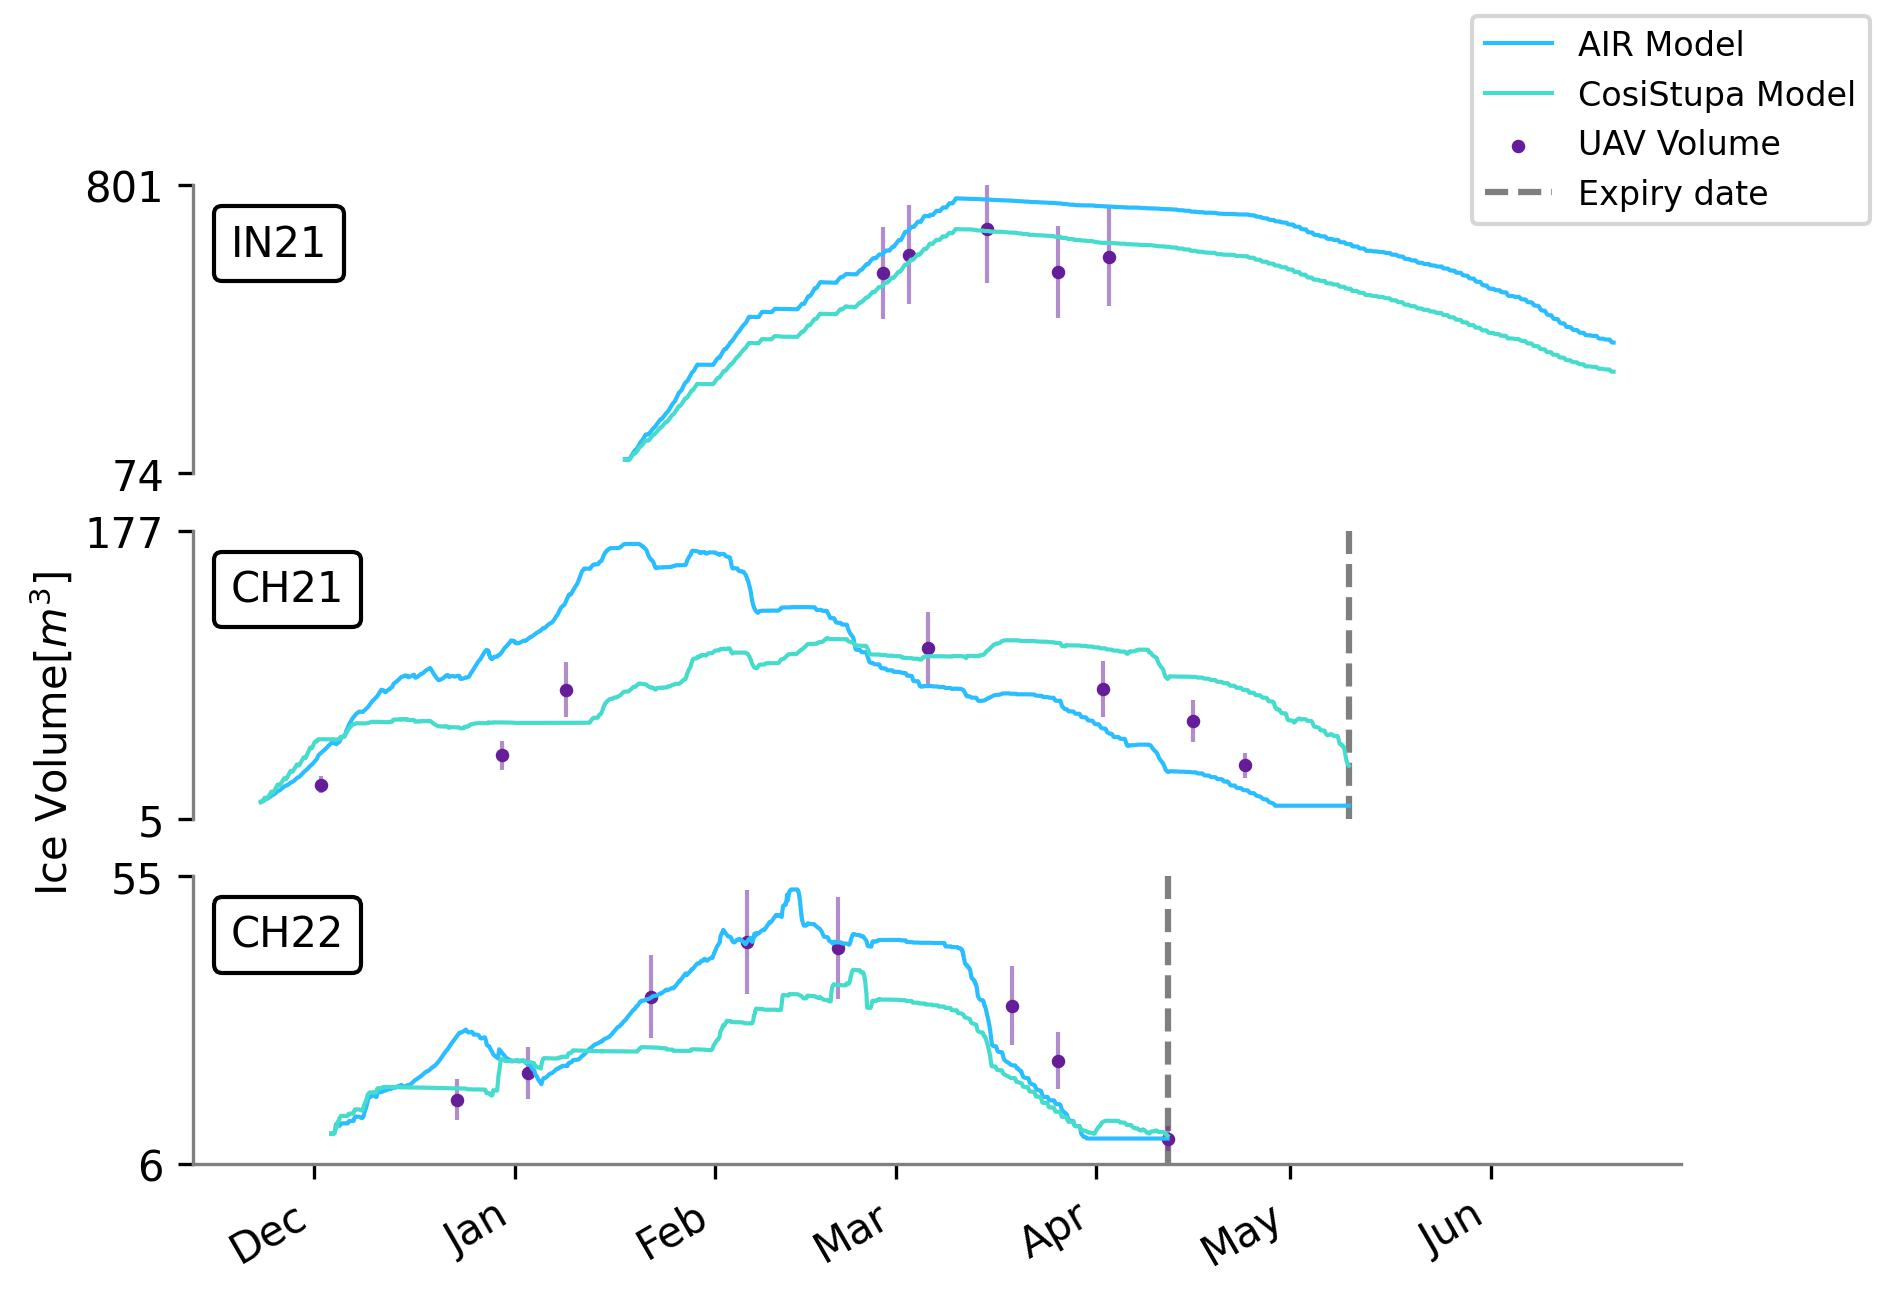
\includegraphics[width=12cm]{Figures/model_compare.jpg}

\caption{}

\label{fig:Cosistupa}
\end{figure}

\section{Suggestions}

\subsection{Model development}

\subsection{Further Data acquisition}

\subsubsection{Meltwater quantities}

\subsubsection{Fountain characteristics}

\subsubsection{Drone flight analysis}

\subsection{Improvement of model algorithm}

\subsubsection{Initialisation of model}

\subsubsection{Better model parametrisations}




 % Experimental Setup

\chapter{Habitat of ice reservoirs}

AIRs cannot be built anywhere. They require a water source sufficiently above and weather conditions cold enough
to amass a seasonal stock of ice. This imposes several meteorological and topographical  requirements for the
chosen construction location. The meteorological requirements can be used to identify favourable regions
worldwide whereas the topographical requirements can be used to pinpoint the construction site within the
respective region. Below we detail these requirements and propose methodologies for finding construction sites
satisfying them. 

\section{Requirements for AIR construction}

\subsection{Meteorological requirements}

AIRs prefer colder, drier and less-cloudy regions. Our results quantify this preference based on maximum ice
volume estimations of the Swiss and the Indian AIRs (see Paper I). The Swiss AIRs have little utility as a water
reservoir due to their small size and short survival duration. Therefore, construction of AIRs should not be
carried out in locations less favourable than the Swiss site. 


\subsection{Topographical requirements}

The water source of an AIR could be either a spring, stream or lake. Springs are the ideal water source since
they are easy to transport via pipelines to the construction site due to their relatively warm temperatures.
Other water sources tend to freeze within the pipeline during tranport. It is pointless to use lakes as water
sources unless there is utility in draining and converting them to ice structures. This is the case for glacial
lakes which can be drained to prevent flash floods while using the water supply to harvest ice structures.

AIRs prefer shadowed valleys. This is because their melt rate is driven by solar radiation (see Paper I).

\section{Quantifying AIR construction potential of any locations}

However, it is challenging to determine a methodology to compare meteorological conditions of two locations. Our
suggested methodology is described in

% \section{Natural vs Artificial Ice Reservoirs}
 % Influence of location

\chapter{Technology of ice reservoirs}

AIRs are a natural evolution of Ladakh's agricultural system. They can be related to traditional water
harvesting technologies like the {\it zing}, which are small tanks where meltwater is collected through the use
of an intricate network of channels. The mountain oases of the Hindu Kush and Karakoram ranges
have similar irrigation networks \citep{nusserLocalKnowledgeGlobal2016}.

\begin{figure}[t]
\centering
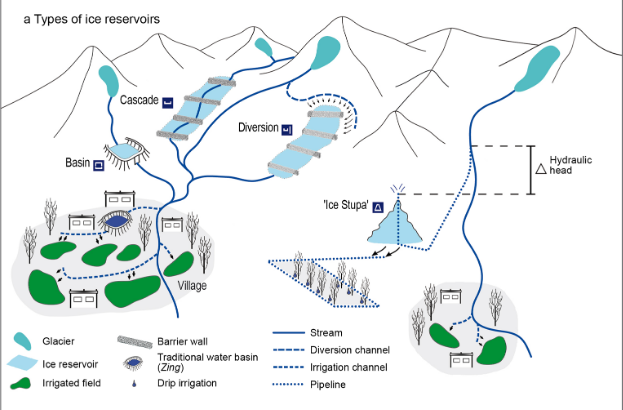
\includegraphics[width=12cm]{Figures/AIR_designs.png}

\caption{Adapted from: \cite{nusserSociohydrologyArtificialGlaciers2019}}

\label{fig:AIRdesigns}
\end{figure}

\section{Ice terraces}


\begin{figure}[t]
\centering
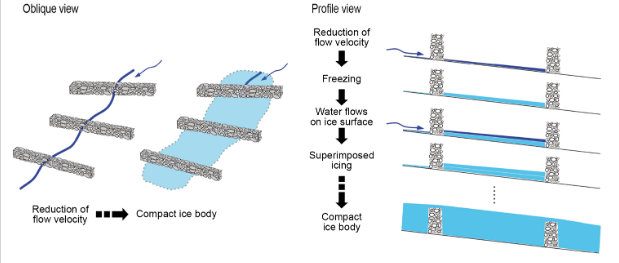
\includegraphics[width=12cm]{Figures/IT_science.png}

\caption{ The process of ice accumulation for ice terraces Adapted from:
\cite{nusserSociohydrologyArtificialGlaciers2019}}

\label{fig:ITscience}
\end{figure}

Ice terraces are the oldest form of AIRs \citep{norphelArtificialGlacierHigh2009}. Usually situated below the
glaciers at elevations where snowmelt starts end of March, these structures facilitate the freezing of stream
water during winter at selected sites, usually shaded by surrounding mountains. Chewang Norphel, a well known
engineer of the Leh Nutrition Project, introduced this practice to Ladakh in the 1980s and 1990s
\citep{vinceGlacierMan2009}.

\subsection{Construction strategy}

There are four distinct types of ice terraces with site-specific modifications as shown in Fig.
\ref{fig:AIRdesigns}: the first type is built as cascades on perennial streams. A series of loose rock walls in
the river bed reduce reduces flow velocity, but still lets water pass through. Such cascades allow flowing water
to freeze on exposed surfaces and form superimposed ice layers when temperatures drop. 

The second type diverts water from streams with higher flow velocity to small side valleys, shaded by
surrounding mountains. This design allows to integrate higher slope positions for additional ice formation. It
consists of a series of partially cemented stone walls across the stream bed. Their dimensions are adjusted
based on the valley topography. The water for the ice terrace is obtained through a long diversion channel. 

The third type is a basin structure, resembling the traditional {\it zing} form of water storage, but located
above the cultivated fields.

\subsection{Application}

\begin{figure}[t]
\centering
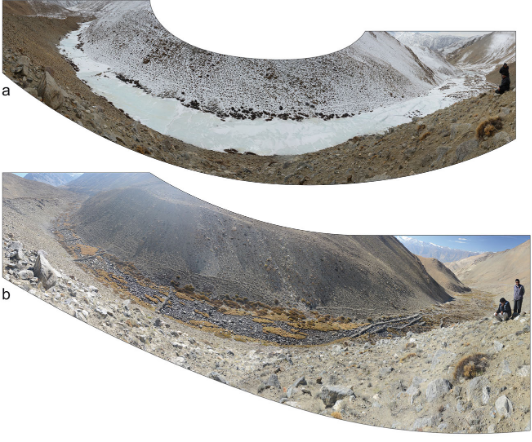
\includegraphics[width=12cm]{Figures/IT_example.png}

\caption{Ice terrace of Phuktse, viewpoint 4430 m. (a) February 2014 (b) October 2014 Adapted from: \cite{nusserSociohydrologyArtificialGlaciers2019}}

\label{fig:ITexample}
\end{figure}

Over the past 30 years, 14 ice terraces have been constructed in central Ladakh, located in tributary valleys of
the Indus. The oldest ice terrace was of the form cascades in Ladakh was built in 1987 at a favourable location
between 4290 and 4640 $m$ in Phuktse. However, according to oral history and Corona imagery from 1969, the first ice
terrace of this design type are older than 50 years and can be found in Phuktse and Igoo. In February 2014,
Phuktse built a successful cascade with an almost continuous stretch of ice (Fig.).


\subsection{Drawbacks}

However, the location requirements and the construction cost of ice terraces were prohibitive for widespread
adoption. 


\section{Ice stupas}

\begin{figure}[t]
\centering
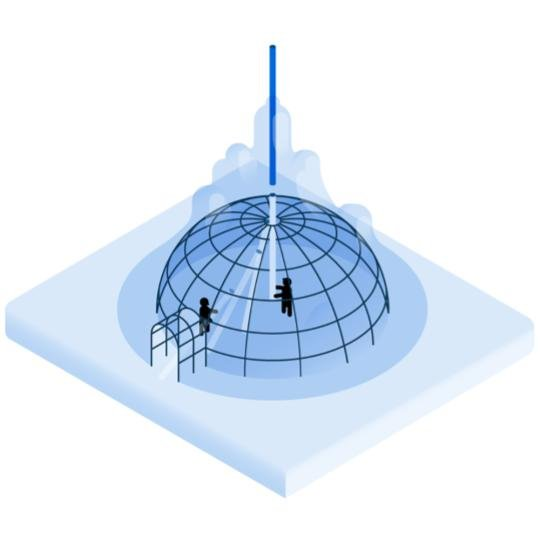
\includegraphics[width=12cm]{Figures/IS_science.jpg}

\caption{ The process of ice accumulation for ice stupas. Diagram by: Francesco Muzzi }

\label{fig:ISscience}
\end{figure}

This prompted the invention of Ice stupas by Sonam Wangchuk in 2013 \ref{wangchukIceStupaArtificial2014}. Due to
their shape, Ice stupas could be built adjacent to the irrigated plantations. It was also relatively cheaper. A
typical Ice stupa just requires a fountain nozzle mounted on a supply pipeline. The water source is usually a
spring or a glacial stream. Due to the altitude difference between the pipeline input and fountain output, water
ejects from the fountain nozzle as droplets that eventually lose their energy and accumulate as ice.  The
fountain is manually activated during the winter nights and is raised, through addition of metal pipes, when
significant ice accumulates below.

\subsection{Construction strategy}

A typical AIR (see Fig. \ref{fig:IS_example}) simply requires a fountain nozzle mounted on a supply pipeline.
The water source is usually a high altitude lake or glacial stream. Due to the altitude difference between the
pipeline input and fountain output, water ejects from the fountain nozzle as droplets which freeze under subzero
winter conditions. The fountain is manually activated during winter nights. The fountain nozzle is raised
through the addition of metal pipes when significant ice accumulates below.  Typically, a dome of branches is
constructed around the metal pipes so that pipe extensions can be done from within this dome. Threads, tree
branches and fishing nets are used to guide and accelerate the ice formation.

\subsection{Application}

\begin{figure}[t]
\centering
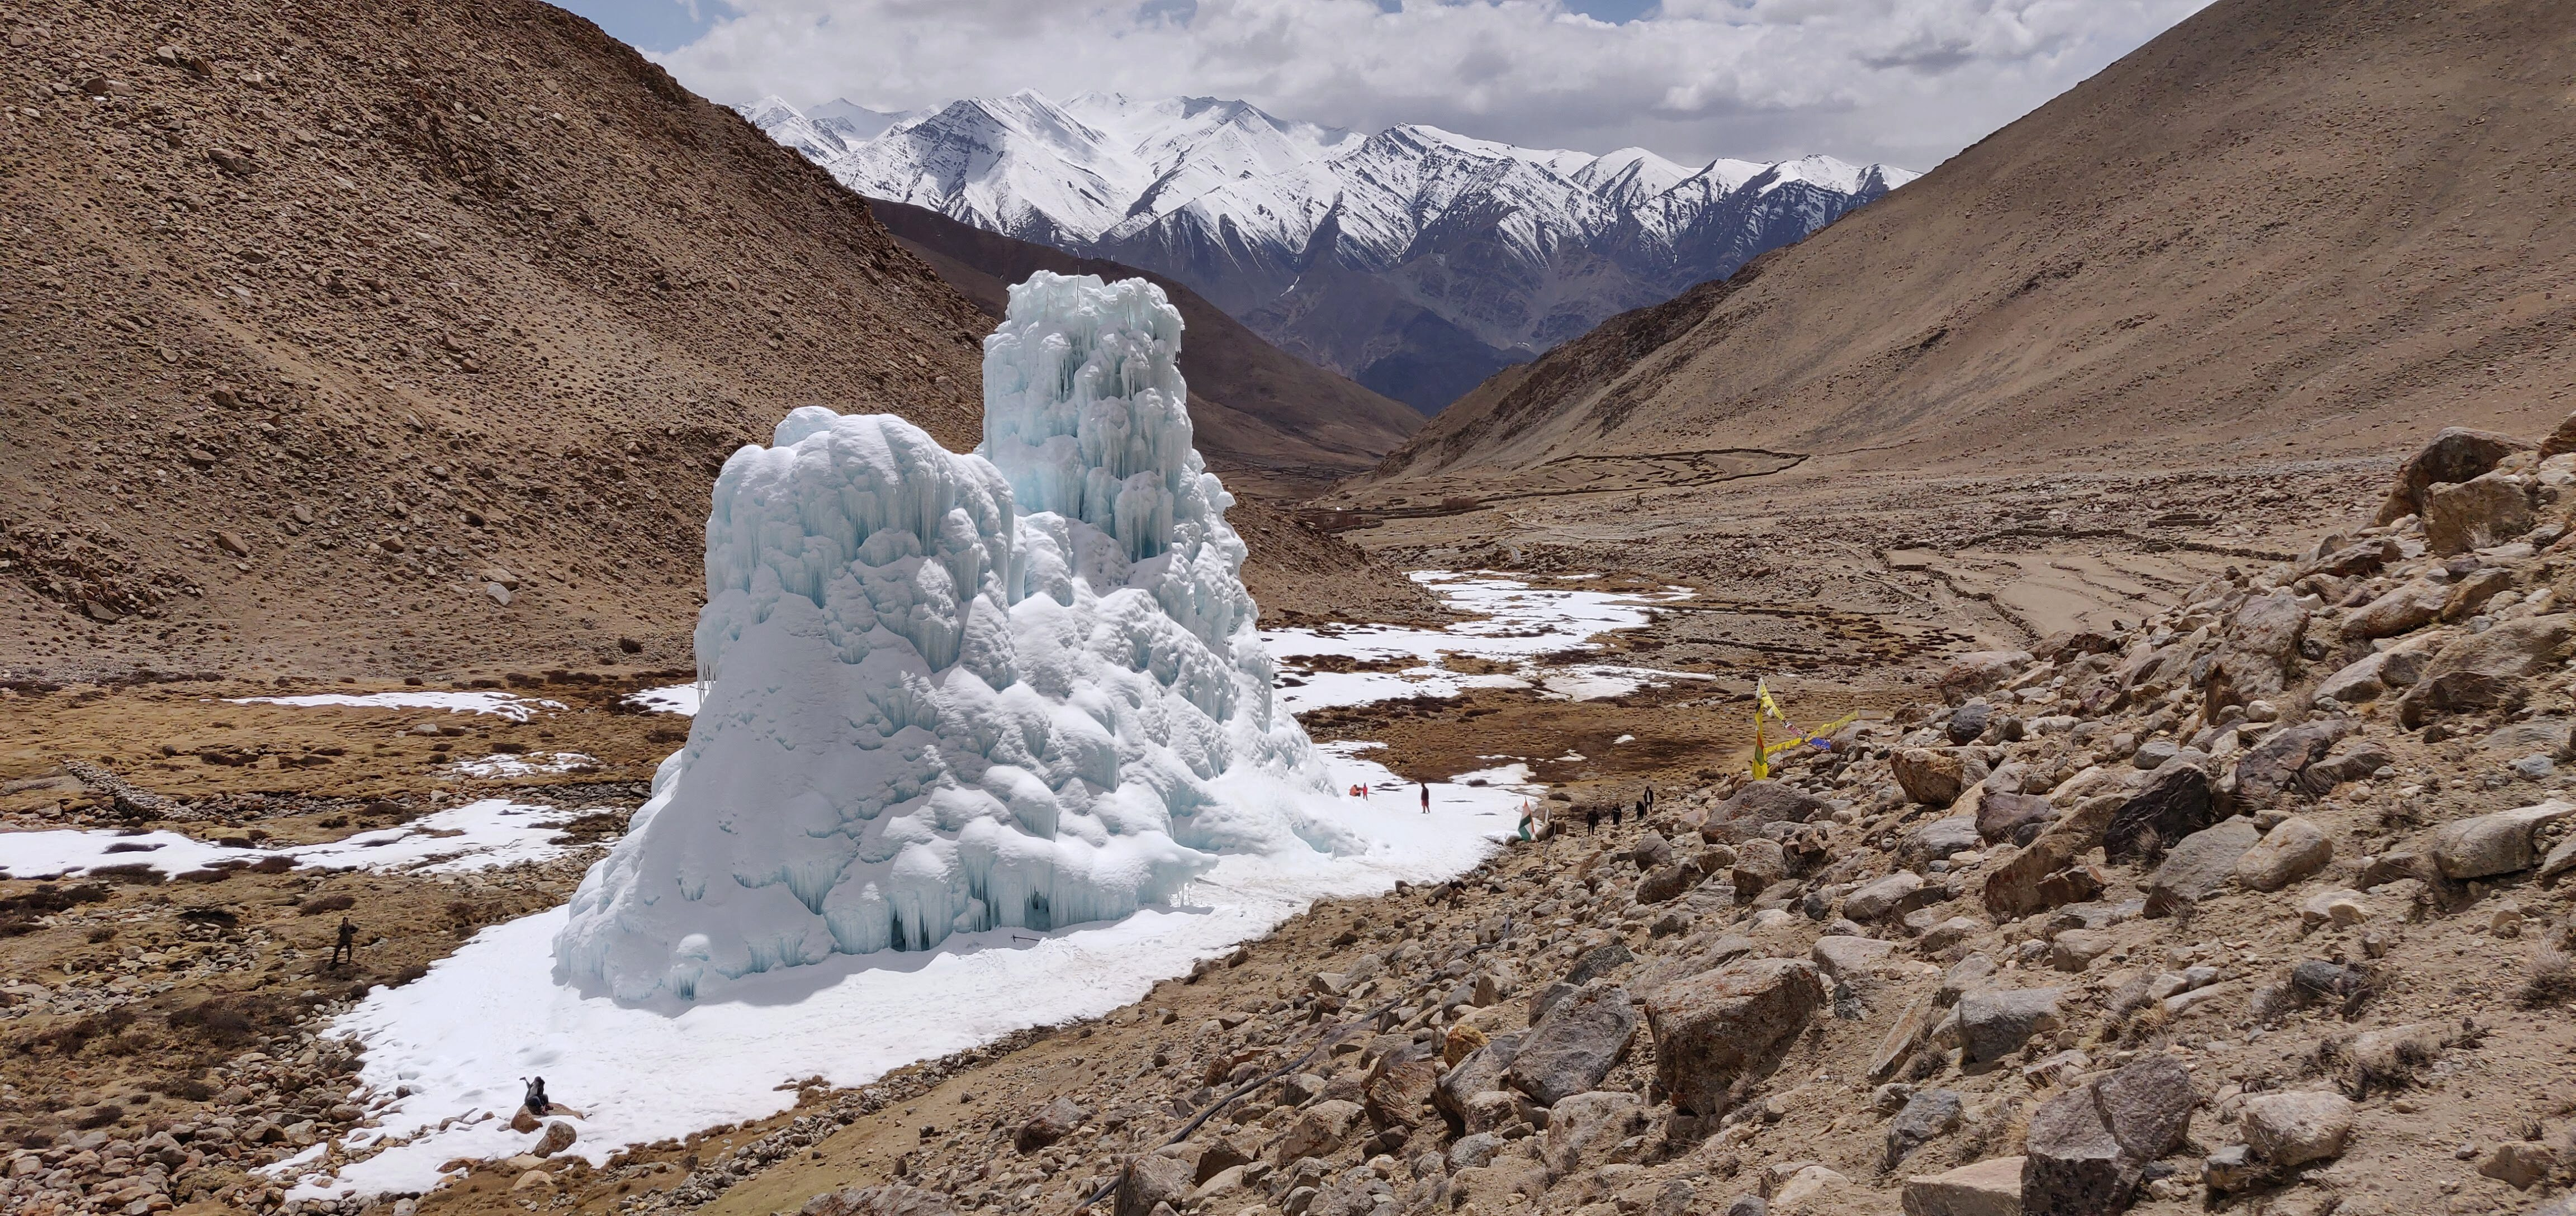
\includegraphics[width=12cm]{Figures/IS_example.jpg}

\caption{Ice terrace of Phuktse, viewpoint 4430 m. (a) February 2014 (b) October 2014 Adapted from: \cite{nusserSociohydrologyArtificialGlaciers2019}}

\label{fig:ISexample}
\end{figure}

\subsection{Drawbacks}

\section{Improvement of construction strategies through weather-sensitive automation systems}

 % Influence of fountain

% \chapter{Design of ice reservoirs}

For centuries, in the Himalayan mountain ranges, local cultures have believed that glaciers are alive. And
what’s more, that certain glaciers can have different genders including male and female. These people ‘breed’
new glaciers by grafting together—or marrying—fragments of ice from male and female glaciers, then covering them
with charcoal, wheat husks, cloths, or willow branches so they can reproduce in privacy. These glacierets
transform into fully active glaciers that grow each year with additional snowfall. Those then serve as lasting
reserves of water that farmers can use to irrigate their crops. Over the years, these practices have inspired
other cultures, where people are creating their own artificial ice reservoirs (AIRs) and applying them to solve
serious modern challenges around water supplies.
 % Influence of design

\chapter{Heritage of ice reservoirs}

Chapter 5 provides conclusions based on research findings from data collected on AIRs in Switzerland and India,
as well as discussion and recommendations for future research. This Chapter will review the purpose of the
study, research questions, literature review, and findings of the study. It will then present conclusions,
discussion of the conclusions, and recommendations for practice and for further research.

\section{Summary}

Cryosphere fed irrigation networks are completely dependant on the timely availability of meltwater from
glaciers, snow and permafrost. With the accelerated decline of glaciers, these irrigation networks have failed
to deliver adequate water to sustain agricultural output and take advantage of the complete growing season. As a
consequence, many mountain villages have either been abandoned or lie on the brink of desertification.

In the past few decades, artificial ice reservoir (AIR) technologies have provided much needed relief to these
water-stressed communities. These strategies revolve around augmenting their glacial ice reservoirs with
man-made ones that provide supplementary irrigation during the spring. 

Summary of the literature review

From folklore to science, from art to technology, these practices of reclaiming glacial water have come a long
way. 

Empirical data and studies focussing on AIRs are sparse. Depending on the relative influence of weather
conditions and fountain characteristics, AIRs typically show high variability in their ice volume dynamics.
Because small-scale processes, complex feedbacks and non-linearities govern their evolution, accessing the
response of AIRs to the location and fountain chosen is challenging and only feasible if backed up with
comprehensive field data. 

Summary of the methodology

In the context of the observed present and predicted global glacier shrinkage, the development of such water
storage technologies is crucial to ensure continued survival of mountain communities.

Summary of the findings

\section{Conclusions}

The main objective of this thesis was thus to improve our understanding about the response of AIRs to changes in
their construction location and fountain characteristics. With a special focus on icestupas, here defined as
vertical AIRs, volume changes were investigated in detail based on the comparison of weather patterns, fountain
characteristics and volume observations between several AIRs. A mass and energy model was created which allowed
ice volume estimation of icestupas. AIR radius, area and volume were recorded using DEMs produced from drone
flights. The fountain characteristics were calibrated from the observed radius and discharge rates. The model
parameters were calibrated from some volume observations. The rest of this DEM dataset were used to validate the
modelled volume evolution. The ice volume dynamics due to the difference in weather patterns of the Swiss
location and Indian location can be summarised as follows: 

% \begin{itemize} 

% \item[\tiny{$\blacksquare$}] Colder temperatures and lower humidity led to higher sublimation and lower
%   conduction.
%  
% \item[\tiny{$\blacksquare$}] Cloudy days increase shortwave radiation impact.
%  
% \end{itemize}

\begin{itemize} 

\item[\tiny{$\blacksquare$}] Icestupa's volume evolution depends on meteorological conditions and fountain
  characteristics.

\item[\tiny{$\blacksquare$}] Icestupas gain volume due to higher vapour losses and not inspite of it. 

\item[\tiny{$\blacksquare$}] Icestupa's shape decreases direct shortwave radiation impact.

\item[\tiny{$\blacksquare$}] Icestupas gain volume due to higher vapour losses and not inspite of it. 

\item[\tiny{$\blacksquare$}] Icestupas suffer high water losses.
 
\end{itemize}

\begin{itemize} 

\item[\tiny{$\blacksquare$}] Colder, drier and less cloudy construction locations form long-lasting AIRs with
  higher maximum ice volumes. 

\item[\tiny{$\blacksquare$}] Fountains that produce smaller droplets form larger AIRs with higher slope. 

\end{itemize}


\section{Discussion}

\section{Recommendations}

\section{Suggestions for future research}

\section{Final thoughts}
 % Conclusion

%% ----------------------------------------------------------------
% Now begin the Appendices, including them as separate files

\addtocontents{toc}{\vspace{2em}} % Add a gap in the Contents, for aesthetics

\lhead{\emph{Symbols}}  % Set the left side page header to "Symbols"
\listofnomenclature{lll}  % Include a list of Symbols (a three column table)
{
% symbol & name & unit \\
$a$ & distance & m \\
$P$ & power & W (Js$^{-1}$) \\
& & \\ % Gap to separate the Roman symbols from the Greek
$\omega$ & angular frequency & rads$^{-1}$ \\
}

%% ----------------------------------------------------------------
\lhead{\emph{List of Figures}}  % Set the left side page header to "List if Figures"
\listoffigures  % Write out the List of Figures

%% ----------------------------------------------------------------
\lhead{\emph{List of Tables}}  % Set the left side page header to "List of Tables"
\listoftables  % Write out the List of Tables

%% ----------------------------------------------------------------
\setstretch{1.5}  % Set the line spacing to 1.5, this makes the following tables easier to read
\clearpage  % Start a new page
\lhead{\emph{Abbreviations}}  % Set the left side page header to "Abbreviations"
\listofsymbols{ll}  % Include a list of Abbreviations (a table of two columns)
{
\textbf{AIR} & \textbf{A}rtificial \textbf{I}ce \textbf{R}eservoirs \\
\textbf{SAIR} & \textbf{S}easonal \textbf{A}rtificial \textbf{I}ce \textbf{R}eservoirs \\
\textbf{PAIR} & \textbf{P}erpetual \textbf{A}rtificial \textbf{I}ce \textbf{R}eservoirs \\
\textbf{HAIR} & \textbf{H}orizontal \textbf{A}rtificial \textbf{I}ce \textbf{R}eservoirs \\
\textbf{VAIR} & \textbf{V}ertical \textbf{A}rtificial \textbf{I}ce \textbf{R}eservoirs \\

}

%% ----------------------------------------------------------------
\clearpage  % Start a new page
\lhead{\emph{Physical Constants}}  % Set the left side page header to "Physical Constants"
\listofconstants{lrcl}  % Include a list of Physical Constants (a four column table)
{
% Constant Name & Symbol & = & Constant Value (with units) \\
Speed of Light & $c$ & $=$ & $2.997\ 924\ 58\times10^{8}\ \mbox{ms}^{-\mbox{s}}$ (exact)\\

}

%% ----------------------------------------------------------------
\clearpage  %Start a new page


% The Acknowledgements page, for thanking everyone
\acknowledgements{
\addtocontents{toc}{\vspace{1em}}  % Add a gap in the Contents, for aesthetics

The acknowledgements and the people to thank go here, don't forget to include your project advisor\ldots

}
\clearpage  % End of the Acknowledgements

\appendix % Cue to tell LaTeX that the following 'chapters' are Appendices

% \chapter{An Appendix}

Lorem ipsum dolor sit amet, consectetur adipiscing elit. Vivamus at pulvinar nisi. Phasellus hendrerit, diam placerat interdum iaculis, mauris justo cursus risus, in viverra purus eros at ligula. Ut metus justo, consequat a tristique posuere, laoreet nec nibh. Etiam et scelerisque mauris. Phasellus vel massa magna. Ut non neque id tortor pharetra bibendum vitae sit amet nisi. Duis nec quam quam, sed euismod justo. Pellentesque eu tellus vitae ante tempus malesuada. Nunc accumsan, quam in congue consequat, lectus lectus dapibus erat, id aliquet urna neque at massa. Nulla facilisi. Morbi ullamcorper eleifend posuere. Donec libero leo, faucibus nec bibendum at, mattis et urna. Proin consectetur, nunc ut imperdiet lobortis, magna neque tincidunt lectus, id iaculis nisi justo id nibh. Pellentesque vel sem in erat vulputate faucibus molestie ut lorem.

Quisque tristique urna in lorem laoreet at laoreet quam congue. Donec dolor turpis, blandit non imperdiet aliquet, blandit et felis. In lorem nisi, pretium sit amet vestibulum sed, tempus et sem. Proin non ante turpis. Nulla imperdiet fringilla convallis. Vivamus vel bibendum nisl. Pellentesque justo lectus, molestie vel luctus sed, lobortis in libero. Nulla facilisi. Aliquam erat volutpat. Suspendisse vitae nunc nunc. Sed aliquet est suscipit sapien rhoncus non adipiscing nibh consequat. Aliquam metus urna, faucibus eu vulputate non, luctus eu justo.

Donec urna leo, vulputate vitae porta eu, vehicula blandit libero. Phasellus eget massa et leo condimentum mollis. Nullam molestie, justo at pellentesque vulputate, sapien velit ornare diam, nec gravida lacus augue non diam. Integer mattis lacus id libero ultrices sit amet mollis neque molestie. Integer ut leo eget mi volutpat congue. Vivamus sodales, turpis id venenatis placerat, tellus purus adipiscing magna, eu aliquam nibh dolor id nibh. Pellentesque habitant morbi tristique senectus et netus et malesuada fames ac turpis egestas. Sed cursus convallis quam nec vehicula. Sed vulputate neque eget odio fringilla ac sodales urna feugiat.

Phasellus nisi quam, volutpat non ullamcorper eget, congue fringilla leo. Cras et erat et nibh placerat commodo id ornare est. Nulla facilisi. Aenean pulvinar scelerisque eros eget interdum. Nunc pulvinar magna ut felis varius in hendrerit dolor accumsan. Nunc pellentesque magna quis magna bibendum non laoreet erat tincidunt. Nulla facilisi.

Duis eget massa sem, gravida interdum ipsum. Nulla nunc nisl, hendrerit sit amet commodo vel, varius id tellus. Lorem ipsum dolor sit amet, consectetur adipiscing elit. Nunc ac dolor est. Suspendisse ultrices tincidunt metus eget accumsan. Nullam facilisis, justo vitae convallis sollicitudin, eros augue malesuada metus, nec sagittis diam nibh ut sapien. Duis blandit lectus vitae lorem aliquam nec euismod nisi volutpat. Vestibulum ornare dictum tortor, at faucibus justo tempor non. Nulla facilisi. Cras non massa nunc, eget euismod purus. Nunc metus ipsum, euismod a consectetur vel, hendrerit nec nunc.	% Appendix Title

%\input{Appendices/AppendixB} % Appendix Title

%\input{Appendices/AppendixC} % Appendix Title

\addtocontents{toc}{\vspace{2em}}  % Add a gap in the Contents, for aesthetics
\backmatter

%% ----------------------------------------------------------------
\label{Bibliography}
\lhead{\emph{Bibliography}}  % Change the left side page header to "Bibliography"
\bibliographystyle{unsrtnat}  % Use the "unsrtnat" BibTeX style for formatting the Bibliography
\bibliography{zot_refs}  % The references (bibliography) information are stored in the file named "Bibliography.bib"

\end{document}  % The End
%% ----------------------------------------------------------------
